\section{Résumé en français}

Ce chapitre s'appuie sur l'article \textit{"Numerical Modeling of Hydraulic Control, Solitary Waves and Primary Instabilities in the Strait of Gibraltar"} \citep{hilt_2020} publié dans la revue \textit{Ocean Modelling}. Si la démarche numérique présentée dans cet article avait été proposée lors de mon stage de fin d'étude, la rédaction même de l'article ainsi qu'une grande majorité des éléments d'analyses présentés (décomposition en valeurs singulières, tests de sensibilité...) ont été réalisés durant la première année de mon doctorat. Ces travaux constituent un véritable socle sur lequel est appuyé le reste de l'étude menée à bien durant ma thèse de doctorat, et sont référencés dans le reste du manuscrit, d'où leur inclusion.

Une configuration numérique simplifiée basée sur une section verticale (2D) est implémentée dans le détroit de Gibraltar avec le code communautaire à surface libre CROCO dans sa version non-hydrostatique, compressible, non-Boussinesq (voir section \noparref{section_croco}). Cette configuration est peu coûteuse en temps de calcul malgré sa haute résolution (environ 45 m sur l'horizontale) et s'appuie sur une bathymétrie réaliste le long de l'axe du détroit avec sa configuration de seuils ( \citet{FA1988}, programme \textit{Gibraltar Experiment}). Durant l'élaboration de cette configuration, une attention toute particulière a été apportée à l'impact de la pseudo-force de Coriolis sur l'échange moyen simulé lors de l'initialisation.

La simulation est initialisée par \textit{lock-exchange} : deux profils de stratification type 'nord Atlantique' et 'Méditerranéen' sont choisis pour initialiser cette configuration simplifiée de part et d'autre du seuil de Camarinal, point central du passage du détroit. Au début de la simulation, le front au-dessus du seuil évolue rapidement en un écoulement bicouche avec des eaux méditerranéennes s'écoulant en courant de gravité dans la moitié ouest du domaine et une intrusion en surface des eaux atlantiques sur la partie est. 

Après une période de simulation d'ajustement de trois jours, la marée semi-diurne est ajoutée par un courant barotrope oscillant à la frontière ouest. Dans une simulation où la rotation de la Terre n'est pas prise en compte, le mélange induit par les courants de marée détruit la stratification obtenue après relaxation du \textit{lock exhange}, modifiant en particulier la profondeur de l'interface où se propagent les solitons. Lorsque la pseudo-force de Coriolis est introduite en même temps que le forçage par la marée, la stratification induite par le mécanisme de \textit{lock-exchange} se maintient, au détriment de la valeur moyennée dans le temps de l'échange au niveau du seuil de Camarinal.

Durant quelques périodes de marée M2, cette configuration simplifiée  permet donc de simuler explicitement et de façon réaliste les variations des processus à l'oeuvre dans le détroit à l'échelle de la marée, et en particulier les processus de fines échelles : propagation de trains d'ondes solitaires, contrôles hydrauliques aux seuils, ressauts hydrauliques internes et mélange turbulent avec la simulation explicite d'instabilités primaires de cisaillement qui ont un effet local sur la stratification. 

Ainsi les ondes internes de grande amplitude de mode 1 se propageant dans l'est du détroit sont caractérisées comme étant des ondes solitaires (ou solitons) par comparaison avec le modèle analytique non-linéaire de Korteweg de Vries. 

La modulation des phénomènes observés par divers paramètres (bathymétrie, intensité des courants de marée, hypothèse hydrostatique, résolution spatiale) est étudiée en détail. A haute résolution (environ 45 m), la relaxation de l'hypothèse non-hydrostatique est indispensable pour représenter les instabilités de cisaillement qui apparaissent dans le jet Méditerranéen, et qui constituent l'amorce de la cascade turbulente directe.

Malgré les défauts inhérents à une représentation 2D-verticale (nécessairement limitée dynamiquement et non représentative des effets longitudinaux comme le contrôle hydraulique dans le détroit de Tarifa), la configuration proposée permet de représenter de façon réaliste et de proposer une première analyse des mécanismes de \textit{fine échelle} dans le détroit à la fréquence de la marée barotrope.



\section{Numerical Modeling of Hydraulic Control, Solitary Waves and Primary Instabilities in the Strait of Gibraltar}
\label{sectionSim2D}
%\author[affilLA]{M. Hilt\corref{mycorrespondingauthor}}\ead{margaux.hilt@aero.obs-mip.fr}
%\address{14 avenue Edouard Belin, 31400 Toulouse, France}
%\author[affilLA]{L. Roblou}
% \author[affilLA]{C. Nguyen}
% \author[affilLEGOSIRD]{P. Marchesiello}
% \author[affilINRIA]{F. Lemari\'e}
%  \author[affilIFREMER]{S. Jullien}
%  \author[affilSHOM]{F. Dumas}
%  \author[affilINRIA]{L. Debreu}
%  \author[affilLOCEAN]{X. Capet}
%  \author[affilSHOM]{L. Bordois}
%  \author[affilLEGOSCNRS]{R. Benshila}
% \author[affilLA]{F. Auclair}

%\cortext[mycorrespondingauthor]{Corresponding author}


%\address[affilLA]{Laboratoire d'A\'erologie, Universit\'e de Toulouse, CNRS, UPS, France}
%\address[affilLEGOSIRD]{LEGOS/IRD, 31400 Toulouse, France}
%\address[affilLEGOSCNRS]{LEGOS/CNRS, 31400 Toulouse, France}
%\address[affilINRIA]{Univ Grenoble Alpes, Inria, CNRS, Grenoble INP, LJK, Grenoble, France}
%\address[affilIFREMER]{Ifremer, Univ. Brest, CNRS, IRD, Laboratoire d'Océanographie Physique et Spatiale (LOPS), IUEM, F- 29280, Plouzan\'e, France}
%\address[affilSHOM]{Service Hydrographie et Oc\'eanographie de la Marine, Brest, France}
%\address[affilLOCEAN]{LOCEAN/IPSL, CNRS/UPMC/IRD/MNHN, Paris, France}


%%%%%%%%%%%%%%%%%%%%%%%%%%%%%%%%%%%%%%%%%%%%%%%%%%%%%%%%%%%%%%%%%%%%%%%%%%%%%%%%%%%%%%%%%

\paragraph{Authors} M. Hilt, L. Roblou, C. Nguyen, P. Marchesiello, F. Lemari\'e, S. Jullien, F. Dumas, L. Debreu, X. Capet, L. Bordois, R. Benshila, F. Auclair

\paragraph{Abstract}
A two-dimensional, vertical section of the Strait of Gibraltar is simulated numerically with the nonhydrostatic / non-Boussinesq three-dimensional CROCO model to investigate details of small-scale dynamics. The proposed configuration is simple, computationally efficient and incorporates the configuration of sills characteristic of this region.
%
Despite the shortcomings of a 2D representation, this configuration provides a realistic depiction of small-scale mechanisms in the strait during a typical tidal cycle: internal solitary waves generation and propagation, occurrence of hydraulic controls and hydraulic jumps at the sills and presence of active turbulent patches. In particular, the well-known eastward propagation of large amplitude internal waves is assessed using the Korteweg de Vries (KdV) propagation model for solitary waves.

As a step towards establishing a realistic three-dimensional Large Eddy Simulation (LES), the sensitivity of the configuration to various choices (e.g., resolution, amplitude of tidal forcing or numerical schemes) is investigated. Our analyses indicate that the representation of small-scale dynamics in the Strait of Gibraltar can be much improved by increasing resolution and relaxing the hydrostatic assumption. Further studies are necessary to grasp the mechanisms of mixing and/or stirring induced by this fine scale processes.
%\end{abstract}

%\begin{keyword}
%Strait of Gibraltar \sep Internal Solitary Waves \sep nonhydrostatic processes \sep Large Eddy Simulation
%\end{keyword}

%\end{frontmatter}

%\linenumbers

%%%%%%%%%%%%%%%%%%%%%%%%%%%%%%%%%%%%%%%%%%%%%%%%%%%%%%%%%%%%%%%%%%%%%%%%%%%%%
\subsection{Introduction}
%%%%%%%%%%%%%%%%%%%%%%%%%%%%%%%%%%%%%%%%%%%%%%%%%%%%%%%%%%%%%%%%%%%%%%%%%%%%%
\begin{figure}[!h]
 \centering
 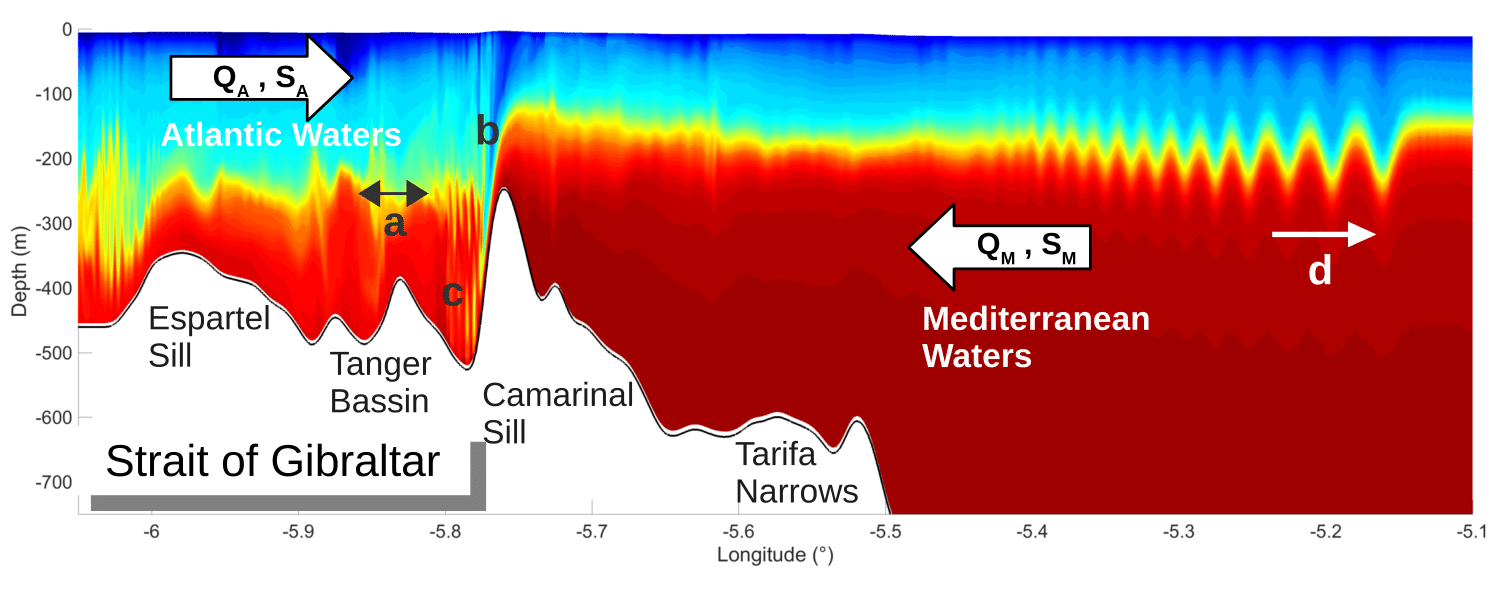
\includegraphics[width=1\textwidth]{./GBR2D/figure1.png}
 \caption{Illustration of small-scale processes in the Strait of Gibraltar induced by tidal interaction with stratification and bathymetry. (a) Linear / Small amplitude internal wave. (b) Hydraulic Jump. (c) Kelvin-Helmholtz instabilities. (d) Large-amplitude internal waves or internal solitary waves (ISW).}
\label{scheme_GBR}
\end{figure}

The Strait of Gibraltar connects two major basins : the Northern Atlantic and the Mediterranean Sea, over which evaporation exceeds precipitation and river run-off. To compensate the resulting loss, exchanges of mass and salt are required through the strait. Figure \ref{scheme_GBR} illustrates the rather complex  exchanges occurring there. %Salty dense Mediterranean water is seen exiting through the Gibraltar strait. 
Inflowing Atlantic water is less salty (salinity $S_A\ \approx\ 36$) than the outflowing Mediterranean water ($S_M\ >\ 38$), and spreads as a surface layer in the Alboran Sea. The interface between the two water masses is distorted by undulations that are not precisely periodic with regard to the tidal cycle but exhibit regularity in some areas.  One of the paper objectives is to better understand the small-scale processes that lead to the Atlantic and Mediterranean water masses transformation in the vicinity of the Strait of Gibraltar.

To further illustrate the exchange between the Northern Atlantic and the Mediterranean, a very simple steady-state model can be expressed as a system of two basic conservation equations.

Volume conservation is expressed as : 
\begin{equation}  
	\label{Eq_mass}
    \displaystyle   
  	Q_A+Q_M = E-P
\end{equation}
while the conservation of salt requires: 
\begin{equation}  
    \label{Eq_salt}
    \displaystyle   
    Q_A S_A + Q_M S_M =  0
\end{equation}

\noindent where $Q_A$ is the Atlantic water volume flux  (positive), $Q_M$ is the Mediterranean water volume flux  (negative), both localized in the Strait of Gibraltar, and $E-P$ is the space-averaged Evaporation minus Precipitation (and river runoff) water budget integrated over the whole Mediterranean Sea. $E-P$ is positive. $S_A$ ($S_M$) stands for Atlantic (Mediterranean) water mean salinity and $ S_M - S_A \approx 2$ \citep{Beth79}. The water budget $E-P$ is positive in the Mediterranean due to excess evaporation that correspond to a yearly averaged loss of water of about 1 meter over the whole basin \citep{Garett90}.

A major dynamical feature in the Strait of Gibraltar is the so-called "flow criticality" usually characterized by the Froude number ($F$): it compares the internal wave phase speed with a flow characteristic velocity. Several definitions of the non-dimensional Froude number can be found in the literature: it can notably be defined for each layer, resulting in a composite number for the whole water column, as in \citet{FA1988} or in \citet{Sannino2009b}. 

A "subcritical" (respectively "supercritical") regime lies in the range of small (respectively large) values of the Froude number $F < 1$ (respectively $F>1$), with an intermediate "critical" regime for $F\approx 1$. The upstream propagation of internal waves is inhibited for supercritical flow so that a hydraulic control occurs at the transition from subcritical to supercritical flow; it persists during periods and within regions of large Froude numbers. As such, the hydraulic regime at a given point will vary in time according to substantial currents variations occurring along the tidal cycle. It is, for example, well established that large amplitude solitary waves in the Strait of Gibraltar can develop due to the hydraulic control at Camarinal Sill \citep{FA1988}, making it a crucial process to represent.

Several analytical models have been proposed to investigate the hydraulic control in the Gibraltar region \citep{BS84,FA1986,Garett90}. The hydraulic control usually occurs in these models at Camarinal Sill (CS), Espartel Sill (ES), and Tarifa Narrows (TN), although the modelled hydraulic control location and frequency vary according to the model refinement :

\begin{enumerate}
\item{\citet{FA1986}'s two-layer model accounts for the strait geometry (depth and width), the exchanged volumes ($Q_A$ and $Q_M$) and the salinity contrast ($S_A -S_M$). This simple model is able to simulate two hydraulic controls: the first one located by the sill, the other in the TN contraction, defining "maximal exchange regime"  (further details are given below). }
\item{In a slightly more elaborated model, the inclusion of entrainment between the two layers and the subsequent interfacial layer introduction modify the left-hand terms of equations \ref{Eq_mass} and \ref{Eq_salt} with the introduction of horizontal and vertical transports in the interfacial layer \citep{Bray95}.  Critical conditions are changed within such two interfaces model which may support two baroclinic modes and new hydraulic controls \citep{Sannino2009b}.}
\item{Considering a three-dimensional flow, the definition of the control needs to account for cross-strait variations such as the tilt of the density interface in the latitudinal direction. In the maximal exchange solution, control in TN may induce the detachment of the surface layer from the northern coast \citep{Sannino2009b}.}
\end{enumerate}

The hydraulic control effect within the strait is illustrated in Figure \ref{scheme_GBR}. The flow is initially subcritical in the Strait; the propagation of internal waves is not hindered at the interface between Atlantic and Mediterranean waters (denoted ``a'' in Figure \ref{scheme_GBR}); then the tidal flood in the vicinity of the Camarinal Sill becomes supercritical. In the supercritical to subcritical transition, downstream of the sill, a "hydraulic jump" (``b'' in Figure \ref{scheme_GBR}) may occur.

Hydraulic jumps are large-amplitude depressions in the regions where hydraulic controls occur. There, intense mixing between the Atlantic and Mediterranean waters takes place as observed by \citet{wesson_1994}. Shear flow instabilities can develop in the hydraulic jump of the Camarinal Sill (denoted ``c'' in Figure \ref{scheme_GBR}). 

The release of hydraulic jumps generates large-amplitude, non-linear, nonhydrostatic Internal Solitary Waves (ISW) trains (denoted ``d'' in Figure \ref{scheme_GBR}) \citep{FA1988}. As the barotropic tide is constrained by the bathymetry, large vertical velocities appear and induce energy transfer to several normal modes of internal waves. Some observations in the Strait of Gibraltar identify the largest ISW amplitude to the first baroclinic mode ; for which vertical velocities have the same direction throughout the water column and all isopycnal surface displacements are in phase. The signature of Mode 2 waves (the vertical velocity profile exhibits one node) has also been observed in the region of Gibraltar strait \citep{FA1988,Vazquez2006}. The internal waves propagate at the interface of Mediterranean and Atlantic waters. 

As the strait flow varies at various timescales during the year, some deviation is expected in the occurrence of the hydraulic control in the strait. This may have a wide impact since local flow conditions combined with the above two conservation equations (\ref{Eq_mass} and \ref{Eq_salt}) determine the relation between the volume fluxes, the evaporation minus precipitation budget ($E-P$) and the salinity difference ($S_A-S_M$) \citep{BK91}. Practically, an "overmixed" solution corresponds to a minimal salinity difference and a maximal exchange of water mass in the strait : it would thus constrict the formation of Mediterranean waters and diapycnal mixing over the Mediterranean basin \citep{BS84,Garett90}. Moreover, the small-scale processes occurring in the strait itself can directly modify the local characteristics of Mediterranean waters \citep{GarciaLafuente2011, Naranjo2015} and Atlantic waters \citep{Millot2014}. This can affect their characteristics as they enter respectively in the North Atlantic sub-basin and in the Mediterranean Sea. 

To study the flow dynamics in the strait in further details, more realistic numerical modelling is of great help. Early attempts used two-layer models  \citep{brandt_1996, Izquierdo2001}. The increase of computational power led to 3D modelling \citep{Sannino2004} with increasing vertical and horizontal resolution, explicitly addressing the tidal cycle and flow characteristics. More recently, even nonhydrostatic models have been used \citep{SG2011, Sannino2014} to explicitly represent the ISW. Other configurations include the Strait of Gibraltar into a Mediterranean circulation model \citep{SN2015}. In this case, the increased resolution locally in the strait \citep{Naranjo2014} --- or the nesting of high-resolution grids within a coarse resolved regional model \citep{Sannino2009} --- shows a clear impact on Mediterranean stratification and improves the representation of convective events in the northwestern Mediterranean basin.

The coastal and regional ocean modelling community model (CROCO\footnote{http://www.croco-ocean.org/}) is based on a new nonhydrostatic and non-Boussinesq solver \citep{Auclair2018} developed within the former ROMS kernel \citep{shchepetkin_regional_2005-1}, for an optimal accuracy and cost efficiency. CROCO opens up new perspectives in terms of modelling of small-scale processes \citep{FoxKemper2019, Lemarie2019}. In this sense, the present study objectives are also numerical: we show that a new generation of nonhydrostatic ocean models can be used efficiently to simulate complex nonlinear, fine scale physics in a realistic but computationally-affordable configuration. The complete solution of Navier-Stokes equations are thus solved numerically for the very first time in a complex realistic regional configuration.


The present configuration of the Strait of Gibraltar is based on a classical lock-exchange initialization \citep{Sannino2002}. A 2D vertical section of the strait is adopted in order to reduce the number of parameters impacting the studied dynamics. 
This rather simple configuration is thus of weak computational cost and reduces the implementation burden; it allows to reach the horizontal and vertical scales of the largest turbulent structures observed in this area. In the strait, where most transverse dynamical feature are an order of magnitude weaker, our numerical approach is some kind of ersatz of a large-eddy simulation (LES\footnote{LES (Large Eddy Simulation): LES, as opposed to DNS (Direct Numerical Simulation) does not cope with the full 3D Kolmogorov energy cascade down to molecular scales. However at least the onset of this cascade (the largest turbulent structures) is explicitly represented, unlike in RANS (Reynolds Averaged Navier-Stokes).}), for which at least the generation process of primary instabilities is correctly represented. However, LES is a 3D concept as the route to molecular dissipation differs in 2D and 3D turbulence. The present study is focused on the description of the largest primary instabilities in the Strait of Gibraltar ; as well as providing order of magnitudes for explicit simulations of these dynamics. Along with these physical aims, the relevance of the chosen numerical methods is a major concern. A quantified impact of the largest turbulent structures on the water masses is out of the scope of what is presented hereafter: it would require a fully three dimensional LES ( also achievable with the CROCO model ), in complement with dedicated relevant experimental measurements.


In Section 2, we present an overview of CROCO equations and the implementation for the 2D lock-exchange experiment. We describe the implementation of the bathymetry profile, water masses, and the exchange and tidal flows. In Section \ref{sRef}, we analyse the physics of the 2D configuration, comparing the model solution to already published data  (e.g., in \citet{FA1988}). Emphasis is then made on the hydraulic control (Section \ref{tide_hyd}), the hydraulic jump (Section \ref{section_insta2D}) and the mode-1 and mode-2 ISW (non-linear internal trains of solitary waves) propagation (Section \ref{sisw}). Last, the sensitivity to the tidal forcing amplitude and to the numerical choices are analysed respectively in sections \ref{TestAmp} and \ref{TestNum}, with a focus on the fine-scales dynamics listed in Figure \ref{scheme_GBR}. 

%%%%%%%%%%%%%%%%%%%%%%%%%%%%%%%%%%%%%%%%%%%%%%%%%%%%%%%%%%%%%%%%%%%%%%%%%%%%%
\subsection{Model Description and Configuration}
%%%%%%%%%%%%%%%%%%%%%%%%%%%%%%%%%%%%%%%%%%%%%%%%%%%%%%%%%%%%%%%%%%%%%%%%%%%%%

%----------------------------------------------------------------------------
\subsubsection{The Numerical Modeling System}
%----------------------------------------------------------------------------

The proposed numerical model of the Strait of Gibraltar simulates explicitly the fine-scale processes (from tens to hundreds of meters) discussed previously. This assumes that (i) a sufficient grid resolution is provided in the strait and (ii) a well-suited numerical kernel is used.

The nonhydrostatic (non-Boussinesq) CROCO version is chosen for its ability to allow the explicit representation of primary instabilities that cascade the kinetic energy injected at large scale down to the smaller scales. This direct transfer ends at the finest scale resolved; the subgrid dissipation of energy is performed both by the implicit mixing of the advection schemes and the explicit closure schemes. The dissipation is solely performed by (quasi-)monotonic numerical advection schemes \citep{Grinstein2007}  when no parametrized turbulent closure scheme accounts for the sugrid-scale mixing.

CROCO is an extension of ROMS from which it inherited the robustness and efficiency of its time-splitting implementation, the accuracy of high-order methods, including its pressure gradient scheme for terrain-following coordinates, and computing performances \citep{shchepetkin_regional_2005-1, Debreu2012, Soufflet2016}. In CROCO's time-splitting algorithm, the "slow mode" is similar to ROMS internal (baroclinic) mode \citep{shchepetkin_regional_2005-1}; its "fast mode" includes the usual external (barotropic) mode and a new pseudo-acoustic mode that allows computation of the nonhydrostatic pressure within a non-Boussinesq formalism \citep{Auclair2018}. A two-level time-splitting kernel is thus conserved in CROCO (as opposed to the first implementation of the 3-level time-splitting by \citet{Auclair2018}) but the fast time step integrates a 3D-compressible flow. Furthermore the slow internal mode is enhanced by a prognostic equation of the vertical velocity, replacing the hydrostatic equation. 

 %----------------------------------------------------------------------------
 \subsubsection{Continuous, Free-Surface, Compressible Equations}
 \label{NavierStokes}
 %----------------------------------------------------------------------------
 
\indent The full set of Navier-Stokes equations for a free-surface ocean is explicitly integrated, including the continuity and momentum equations, the surface kinematic relation, the heat, salt and state equations in Cartesian coordinates : 
\begin{eqnarray}
   %%%%%%%%%%%%%%%%%%%%%%%%%%%%%%%%%%%%%%%%%%%%%%
   % Continuity
   %%%%%%%%%%%%%%%%%%%%%%%%%%%%%%%%%%%%%%%%%%%%%%
   \partial_t\rho &&=-\vec{\nabla}.(\rho\vec{v})\\[3mm]
   %%%%%%%%%%%%%%%%%%%%%%%%%%%%%%%%%%%%%%%%%%%%%%
   % Momentum
   %%%%%%%%%%%%%%%%%%%%%%%%%%%%%%%%%%%%%%%%%%%%%%
   \label{momentum}
   \partial_t\rho\vec{v} &&=
   -\vec{\nabla}.\left(\rho\vec{v}\otimes\vec{v}\right)
   -2\rho\vec{\Omega}\wedge\vec{v}
   -\vec\nabla p+\rho\vec{g}
   +\mu\Delta\vec{v}
   +\lambda\vec{\nabla}(\vec{\nabla}.\vec{v})\\[3mm]
   %%%%%%%%%%%%%%%%%%%%%%%%%%%%%%%%%%%%%%%%%%%%%%
   % Surface kinematic relation
   %%%%%%%%%%%%%%%%%%%%%%%%%%%%%%%%%%%%%%%%%%%%%%
   \partial_t{\zeta} &&= 
   w\scriptstyle(z=\zeta)\textstyle
   -\vec{v}\scriptstyle(z=\zeta)\textstyle.\vec{\nabla}{\zeta}\\[3mm]
   %%%%%%%%%%%%%%%%%%%%%%%%%%%%%%%%%%%%%%%%%%%%%%
   % Heat equation
   %%%%%%%%%%%%%%%%%%%%%%%%%%%%%%%%%%%%%%%%%%%%%%
   \partial_t{\rho\theta} &&=-\vec{\nabla}.\left(\rho\theta\vec{v}\right)
   +\kappa_{\theta}\Delta\theta\\[3mm]
   %%%%%%%%%%%%%%%%%%%%%%%%%%%%%%%%%%%%%%%%%%%%%%
   % Salt equation
   %%%%%%%%%%%%%%%%%%%%%%%%%%%%%%%%%%%%%%%%%%%%%%
   \partial_t{\rho S} &&=-\vec{\nabla}.\left(\rho S\vec{v}\right)
   +\kappa_{S}\Delta S\\[3mm]
   %%%%%%%%%%%%%%%%%%%%%%%%%%%%%%%%%%%%%%%%%%%%%%
   % State equation
   %%%%%%%%%%%%%%%%%%%%%%%%%%%%%%%%%%%%%%%%%%%%%%
   \rho &&=\varrho\left(\theta,S,P\right)
\end{eqnarray}
where $\vec{v}=(u,v,w)$ is the velocity, $p$ the total pressure, $\zeta$ the free-surface anomaly, $\rho$ the density, $\theta$ and $S$ the potential temperature and salinity respectively. $\vec{\Omega}$ is the instantaneous earth rotation vector, $\vec{g}$ is the acceleration of gravity and $\mu$, $\lambda$, $\kappa_{\theta}$ and $\kappa_{S}$ are respectively the dynamical and second (bulk) viscosity and the thermal and salinity diffusivities. $\varrho\left(\theta,S,P\right)$ is a linear approximation of the seawater equation of state. 

   
 %----------------------------------------------------------------------------  
 \subsubsection{Density and Pressure Decomposition}
 %----------------------------------------------------------------------------
\indent As part of the time-splitting, the density is splitted into one slow and one fast component based on a first-order decomposition with respect to the total pressure. In the following, $s$ and $f$ subscripts refer to these slow and fast components respectively.\\
\begin{eqnarray}
   %%%%%%%%%%%%%%%%%%%%%%%%%%%%%%%%%%%%%%%%%%%%%%
   % Density
   %%%%%%%%%%%%%%%%%%%%%%%%%%%%%%%%%%%%%%%%%%%%%%
  \rho &&=\rho_{s}\left(\theta,S,P\right)
  +\overbrace{\left.{\frac{\partial{\rho}}{\partial{P}}}\right|_{\theta,S}\delta{P}}^{\delta{\rho}=\rho_{f}}
  +O\left(\delta{P}^2\right)\\
   %%%%%%%%%%%%%%%%%%%%%%%%%%%%%%%%%%%%%%%%%%%%%%
   % Pressure
   %%%%%%%%%%%%%%%%%%%%%%%%%%%%%%%%%%%%%%%%%%%%%%
  P &&=\underbrace{P_{atm}
  +\int\limits_z^{\zeta}{(\rho_{s}-\rho_0)g\ dz'}}_{Slow\ mode}
  +\underbrace{\rho_{0}g(\zeta-z)+\underbrace{\delta P}_{P_{f}}}_{Fast\ mode}
\end{eqnarray}
  
No further decomposition is required for the other variables. Note that $\delta P$ is the nonhydrostatic pressure.
 
%----------------------------------------------------------------------------  
 \subsubsection{Slow vs Fast Components}
 %----------------------------------------------------------------------------
\indent Navier-Stokes equations are integrated with two different time-steps in a time-splitting algorithm. The slow mode is identical to ROMS whereas the fast mode is now 3D and includes the integration of the compressible terms of the momentum and continuity equations. The free-surface anomaly is computed through the surface kinematic condition.
  
 \begin{eqnarray}  
 \label{NBQsyst}
   %%%%%%%%%%%%%%%%%%%%%%%%%%%%%%%%%%%%%%%%%%%%%%
   % Continuity
   %%%%%%%%%%%%%%%%%%%%%%%%%%%%%%%%%%%%%%%%%%%%%%
   \partial_t\ \rho_f &= -\partial_t\ \rho_{s}
   &-\vec{\nabla}.(\rho\vec{v}) \nonumber \\
   %%%%%%%%%%%%%%%%%%%%%%%%%%%%%%%%%%%%%%%%%%%%%%
   % Momentum
   %%%%%%%%%%%%%%%%%%%%%%%%%%%%%%%%%%%%%%%%%%%%%%
   \partial_t\rho\vec{v} &= 
   & \overbrace{-\vec{\nabla}.\left(\rho\vec{v}\otimes\vec{v}\right)
   -2\rho\vec{\Omega}\wedge\vec{v}
   -\vec\nabla(\int\limits_z^{\zeta_f}{(\rho_{s}-\rho_0)g\ dz'})
   +\mu\Delta\vec{v}}^{\vec{\Lambda}_{s}} \nonumber \\
   &&\underbrace{-\rho_{0}g\vec\nabla\zeta_f
   -\vec\nabla{P}
   +\rho\vec{g}
   +\lambda\vec{\nabla}(\vec{\nabla}.\vec{v})}_{\vec{\Lambda}_{f}}\\
   %%%%%%%%%%%%%%%%%%%%%%%%%%%%%%%%%%%%%%%%%%%%%%
   % Surface kinematic relation
   %%%%%%%%%%%%%%%%%%%%%%%%%%%%%%%%%%%%%%%%%%%%%%
   \partial_t{\zeta_f} &&= 
   w_f\scriptstyle(z=\zeta)\textstyle
   -\vec{v_f}\scriptstyle(z=\zeta)\textstyle.\vec{\nabla}{\zeta_f} \nonumber \\[3mm]
   %%%%%%%%%%%%%%%%%%%%%%%%%%%%%%%%%%%%%%%%%%%%%%
   % Heat equation
   %%%%%%%%%%%%%%%%%%%%%%%%%%%%%%%%%%%%%%%%%%%%%%
   \partial_t{\rho\theta_s} &=\ &\Theta_{s}=-\vec{\nabla}.\left(\rho\theta_s\vec{v}\right)
   +\kappa_{\theta}\Delta\theta_s \nonumber \\
   %%%%%%%%%%%%%%%%%%%%%%%%%%%%%%%%%%%%%%%%%%%%%%
   % Salt equation
   %%%%%%%%%%%%%%%%%%%%%%%%%%%%%%%%%%%%%%%%%%%%%%
   \partial_t{\rho S_s} &= &\ \Sigma_{s}= -\vec{\nabla}.(\rho S_s\vec{v})
   +\kappa_{S}\Delta{S_s} \nonumber \\
   %%%%%%%%%%%%%%%%%%%%%%%%%%%%%%%%%%%%%%%%%%%%%%
   %State equations
   %%%%%%%%%%%%%%%%%%%%%%%%%%%%%%%%%%%%%%%%%%%%%%
   \rho_s &= &\varrho(\theta_s,S_s,\zeta_f) \nonumber \\
   \rho_f &= &c_s^{-2} P_f \nonumber    
 \end{eqnarray} 
 
The momentum equations are integrated both in the slow and fast modes but the right-hand-side of the equation is split in two parts: a "slow" part $(\vec{\Lambda}_{s})$ made of slowly varying terms (advection, Coriolis force, baroclinic pressure force and viscous dissipation) and a "fast" part $(\vec{\Lambda}_{f})$, made of fast-varying terms (the surface-induced and compressible pressure force, the weight and dissipation associated with bulk-viscosity). This momentum equation is numerically integrated twice, once with a large time-step keeping $\vec{\Lambda}_{f}$ constant, and once with a smaller time-step keeping $\vec{\Lambda}_{s}$ constant. This time-splitting is much more computationally efficient than integrating the whole set of equations at the same short time step.% (i.e. constrainted by the pseudo-acoustic wave celerity). 

The general, compressible equations set \ref{NBQsyst} can basically propagate three types of waves: internal and external gravity waves, and acoustic waves propagating at $c_s$, the speed of sound. The nonhydrostatic pressure anomaly is not a solution of a diagnostic elliptic Poisson-like equation as it is for a Boussinesq equations set. The pressure anomalies travel at the acoustic waves velocity. The acoustic solver is not global anymore (as it is in the Poisson-like set); it is now local in space, meaning that no 3D global linear system of equations needs to be inverted anymore. The price of solving fast acoustic waves is however enhanced due to a more restrictive CFL conditions. Both acoustic and surface waves are integrated in CROCO's fast mode with a smaller time-step to cope with this. As a linear set of simplified compressible equations needs to be integrated in this fast mode the whole computations remain affordable. In addition, since the sound speed is at least one order of magnitude larger than the phase-velocity of the fastest propagating waves and much larger than any ocean advection velocity, it can be artificially reduced. The only requirement is that the speed of sound remains larger than any other propagating wave or flow velocity in the domain. In particular, it must remain larger than the phase-velocity of long surface waves so that nonhydrostatic anomalies can be propagated vertically fast enough to set up the corresponding wave structure over the water column. Sensitivity tests show that, in this case, a slower sound speed has no impact on lower-frequency dynamics in the region of the strait: more details on that point can be found in \citet{Auclair2018}. 



%----------------------------------------------------------------------------  
 \subsubsection{Bathymetry}
 \label{BathyNum}
 %----------------------------------------------------------------------------

\begin{figure}[!h]
\centering
 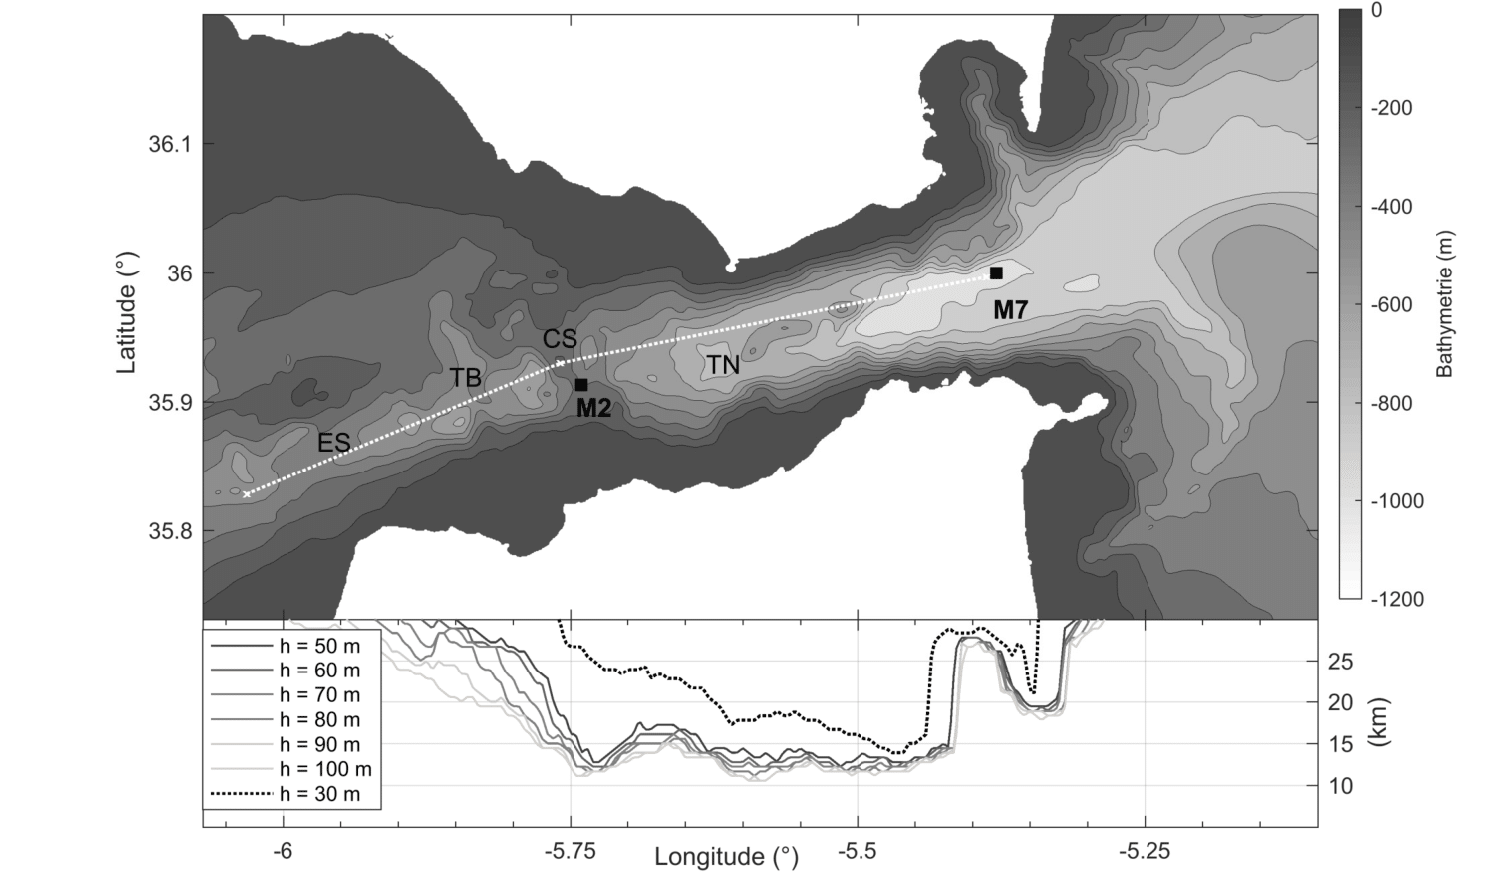
\includegraphics[width=1\textwidth]{./GBR2D/figure2.png}
 \caption { a) Bathymetry of the strait of Gibraltar, with the section used for the present model configuration (white dotted line). Black squares indicate the position of moorings from \citet{CW90}; ES: Espartel Sill, TB: Tanger Basin, CS: Camarinal Sill , TN: Tarifa Narrows. b) Width of the Gibraltar Strait along transverse direction (y) between 2 isobaths of depth h.}
 \label{Fig1}
\end{figure}

\indent Figure \ref{Fig1}.a presents the 500-m-resolution bathymetry gathered in the framework of the HOMONIM project coordinated by the French Navy (SHOM) and MeteoFrance, and as provided by the French Navy \citep{Biscara2016}. The  main bathymetric features as well as the localization of the studied 2D vertical section are exhibited. This section is chosen as close as possible to the transect of Farmer and Armi's Gibraltar Experiment performed in April 1986 \citep{FA1988} and coincides in the western area with the Mediterranean waters privileged path. Hereafter, $u$ is the velocity in the longitudinal direction of the section and $v$ the velocity in the transverse direction. Figure \ref{Fig1}.b presents the Gibraltar Strait width according to different reference depths. This plot shows that an averaged thirteen kilometer width can be used, featuring steep slopes at the lateral boundaries of the strait, especially in Tarifa Narrows.

Simulations are performed with 50m and 220m horizontal resolutions. The bathymetry used in the simulations is averaged laterally to limit the unrealistic effect of local seamounts in the transverse direction such as those found in TN (which can end up acting as another sill in a 2D vertical section). To that end, a Gaussian interpolation of the bathymetry along the section in Figure \ref{Fig1}.a is used with a greater Gaussian radius in the transverse direction than in the longitudinal direction. The Gaussian radius in the transverse direction is set to 1500 m (i.e. lower than the width of the strait in figure \ref{Fig1}.b). As a consequence, the bathymetry only reflects the deepest areas in the canal. In the longitudinal direction, the Gaussian interpolation radius is set to 300 m to preserve the bathymetry variability in this direction.

The minimum depth thus assessed at Camarinal Sill (i.e. the main sill in the Strait), along the transect's path goes from the value of approximately 200 m to 245 m. The model bathymetry used is the one shown in Figure \ref{scheme_GBR}. A reference simulation (hereafter named \textbf{SimRef}) is carried out at 50-m horizontal resolution with additional characteristics and parameters listed in \ref{tabsimref}.

%~

\begin{table}
\caption{Numerical parameters of simulation \textbf{SimRef}}
\centering
\begin{tabular}{|p{0.5\linewidth}|c|c|}
\hline
Number of horizontal points & \multicolumn{2}{c|} {2661x3}  \\
%\hline
Horizontal scale ($\Delta x$) & \multicolumn{2}{c|} {50 m}\\ 
%\hline
Number of vertical $\sigma$-levels & \multicolumn{2}{c|} {40} \\
%\hline
Depth & Min & Max\\
%\cline{2-3}
   & 247 m & 900 m\\
%   \hline
   Vertical scale ($\Delta$z) & 6 m & 23 m\\
%\hline
Slow time step ($t_s$) & \multicolumn{2}{c|} {1 s}\\
%\hline
Fast time step ($t_f$) & \multicolumn{2}{c|} {1/8 s}\\
%\hline
Spin up period & \multicolumn{2}{c|} {72 h}  \\
%
Vertical Viscosity & \multicolumn{2}{c|} {$10^{-6}$ m$^2$/s}\\
%\hline
Lateral Viscosity & \multicolumn{2}{c|} {$10^{-5}$ m$^2$/s}\\
%\hline
Diffusivity & \multicolumn{2}{c|} {$10^{-6}$ m$^2$/s}\\
%\hline
Momentum Advective Scheme & \multicolumn{2}{c|} {TVD - Van Leer}  \\
%\hline
Turbulent Closure Scheme & \multicolumn{2}{c|} {none}  \\
%\hline
T, S Advective Scheme & \multicolumn{2}{c|} {WENO5}  \\
Quadratic bottom drag coefficient & \multicolumn{2}{c|}{$10^{-3}$}\\
Atmospheric forcing/fluxes & \multicolumn{2}{c|}{none}\\
\hline
\end{tabular}
\label{tabsimref}
\end{table}

\begin{figure}[!t]
 \centering
 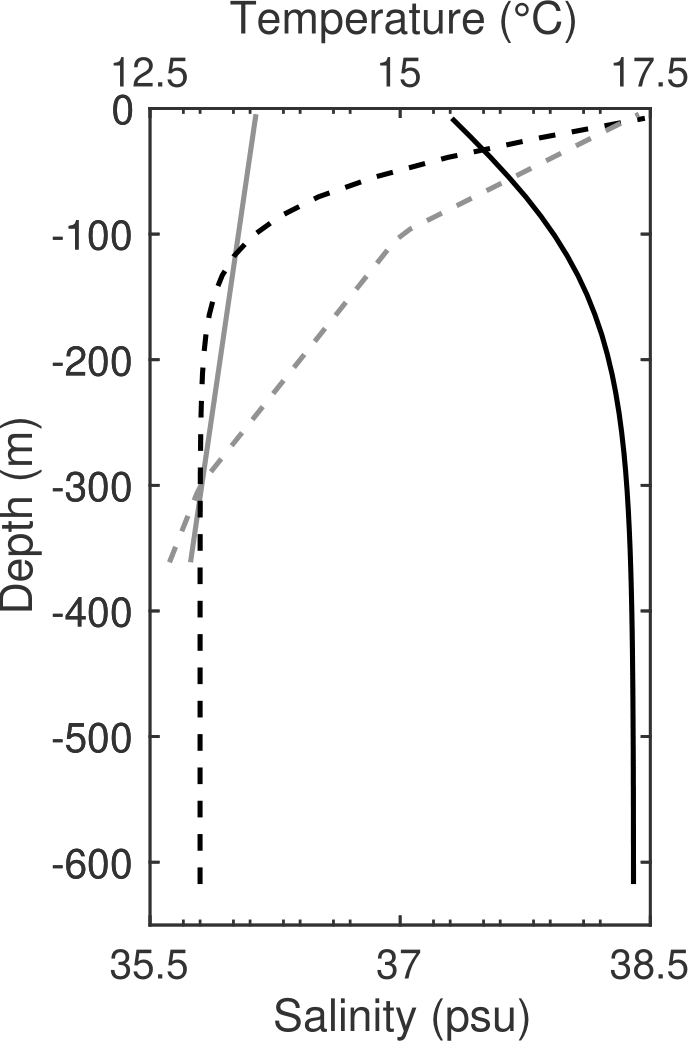
\includegraphics[width=0.5\textwidth]{./GBR2D/figure3.png}
 \caption{Initial salinity (solid) and temperature (dashed) profiles of Mediterranean water (black) and Atlantic water (grey).}
\label{fig_LEx}
\end{figure}


%--------------------------------
\subsubsection{Initial Water Masses, Tidal Forcing and Boundary Conditions}
\label{init}
%--------------------------------
\indent The temperature and salinity reference profiles are chosen to initialise the density field of the simulations. A minimum of two profiles for each of those variables is needed to initialize gradients associated with sloping isopycnal surfaces in a given direction. According to \citet{Sannino2002}, a lock-exchange initialization is performed with homogeneous Atlantic water initially to the west of the CS and homogeneous Mediterranean water to the east. A three-day spin-up described in Section \ref{Coriolis}) is then performed to set up the exchange flow in the strait.

The initial temperature and salinity profiles are presented in Figure \ref{fig_LEx}. The contrast in salinity between Atlantic and Mediterranean waters is noticeable, with respective mean values of 35.9 and 38.2. 

In the following, the interface between Atlantic and Mediterranean layers is taken as the 37 isohaline, following \citet{Bryden94}. Density is now expressed as an anomaly (written $\rho'$) relative to a reference (mean) density $\rho_{0}$. From now on, the implicit reference density (unless contraindicated) will be $\rho_{0}=1033.7$ kg/m$^3$: a value reached in the pycnocline separating the two water masses.

An idealized M2 tidal forcing (of period T = 12.4 h) is prescribed at the open boundaries after the spin-up period (at t = 3 days = 5.8 T ). It is introduced thanks to a barotropic current of amplitude 0.4 m/s at the western boundary (0.8 m/s at CS), corresponding to a moderate regime according to the TPXO-8 tidal atlas \citep{tpxo8}. Lateral forcing is introduced at the open eastern and western boundaries through mixed active passive radiation conditions  \citep{Marchesiello2001} ; cyclic conditions are imposed to the northern and southern open boundaries.

%----------------------------------------------------------------------------
\subsubsection{Initial Flow and Effect of Coriolis Force}
\label{Coriolis}
%----------------------------------------------------------------------------

The Gibraltar strait lateral boundaries  are distant of about 15 km, with a clear funneling effect from the CS to the eastern end of the strait ( 5.4$^\circ$W; see Figure \ref{Fig1}.b). The internal Rossby radius $R$ (\ref{app_Rossby}) is usually found to vary from 10 to 20 km \citep{Bormans1989, CW90, vlasenko_2009}. The width of the strait and the Rossby radius $R$ being of the same order of magnitude, rotational effects can be neglected as a rather good approximation. Therefore, the momentum balance is mainly between the acceleration and the pressure force in the equation (\ref{momentum}) and the geostrophic adjustment in the along-strait direction is locally neglected. In their observations \citep{FA1988} and the 3D-modeling configurations \citep{Sannino2002}, the consequence of Earth's rotation is a cross-strait shear of along-strait velocity \citep{Bormans1989} and a tilt of the isopycnals: along the southern boundary  (i.e. along the Moroccan coast), the interfacial isopycnal is deeper and the flow reaches larger velocities.

As the transverse flow, the coastal boundaries, and the resulting ``funnelling effect'' cannot be simulated in a 2D vertical section, it is necessary to examine whether completely ignoring rotational effects is viable in a 2D vertical approximation. To that end, three different numerical simulations of the stratification and the mean circulation are compared: (i) one simulation with the Coriolis force activated from start to end (\textbf{SimAllCor}; $f = 8.5 \ 10^{-5} s^{-1}$), (ii) the second one without the Coriolis force (\textbf{SimNoCor}; $f=0$), and (iii) the last one with the Coriolis force activated only after a three days spin-up period (\textbf{SimRef}). Apart from the Coriolis parameter, all the three simulations where performed with the characteristics given in Table \ref{tabsimref} for \textbf{SimRef}. During the very first hours of simulation time, the `Lock-Exchange dam' separating the Atlantic and Mediterranean water-masses disappears; a gravity current is generated with dense Mediterranean waters flowing down the western slope of CS and light Atlantic water spreading in the surface layer east of the sill.

Figure \ref{fig2} presents the field of the longitudinal velocity ($u$) as well as some isopycnals for \textbf{SimAllCor} (a) and \textbf{SimNoCor} (b) at t = 72 h (i.e., the end of the spinup period). The bold isopycnal surface $\rho'= -0.7\ kg/m^3$ corresponds at that time to the 37psu-isohaline. Figures \ref{fig2}.a-b  also present the transverse-velocity ($v$) isotachs $\pm$ 0.5 m/s. Figures \ref{fig2}.c-d show the tidal residual components $u$ and $v$ in the water column at the two dashed vertical lines on figures \ref{fig2}.a-b. These locations correspond to the moorings indicated in Figure 1 of \citet{CW90}. Using the 37psu-isohaline as a frontier between the two water masses, the 3T time-averaged transport through the left dashed line at the CS is given in the columns labelled 'Transport' of the Table \ref{tabdepth}.

In \textbf{SimNoCor} (Figure \ref{fig2}.b), a clear vertical shear of the along-section velocity can be seen between the two water masses. The shear is still featured in the 3T-averaged current profiles of Figure \ref{fig2}.c and is, for station M2, in accordance with the observations given by the moorings at the CS. This shear has decreased since initialization as progressive mixing of the two water masses reduces the baroclinicity. The currents in \textbf{SimAllCor} and \textbf{SimRef} are weaker, with locally negative currents in the upper layer (see Figure \ref{fig2}.c). This is confirmed by the layer-averaged transports presented in Table \ref{tabdepth}, where values in \textbf{SimAllCor} and \textbf{SimRef} are one order of magnitude smaller than in \textbf{SimNoCor}. Using an average strait's width of 13 km, an approximate baroclinic transport for the strait can be estimated from the values in Table \ref{tabdepth}; for \textbf{SimNoCor} it would be of 0.6 Sv: it is slightly weaker than the range of 0.7-1 Sv estimated from various field observations (see a review in \citet{Sammartino2015}). In \textbf{SimAllCor} and \textbf{SimRef}, the cross-section velocity is due to the inclusion of the Coriolis force. More precisely, during the spin-up phase of \textbf{SimAllCor}, the effect of rotation can no more be neglected after 6 hours. At that time, the upper Atlantic layer has spread over a distance of about 26 km and the cross-section velocity featured in Figure \ref{fig2}.a is already significant.

%
%%%%%%%%%%%%
% Figure 
%%%%%%%%%%%%
\begin{figure}
% \centering
 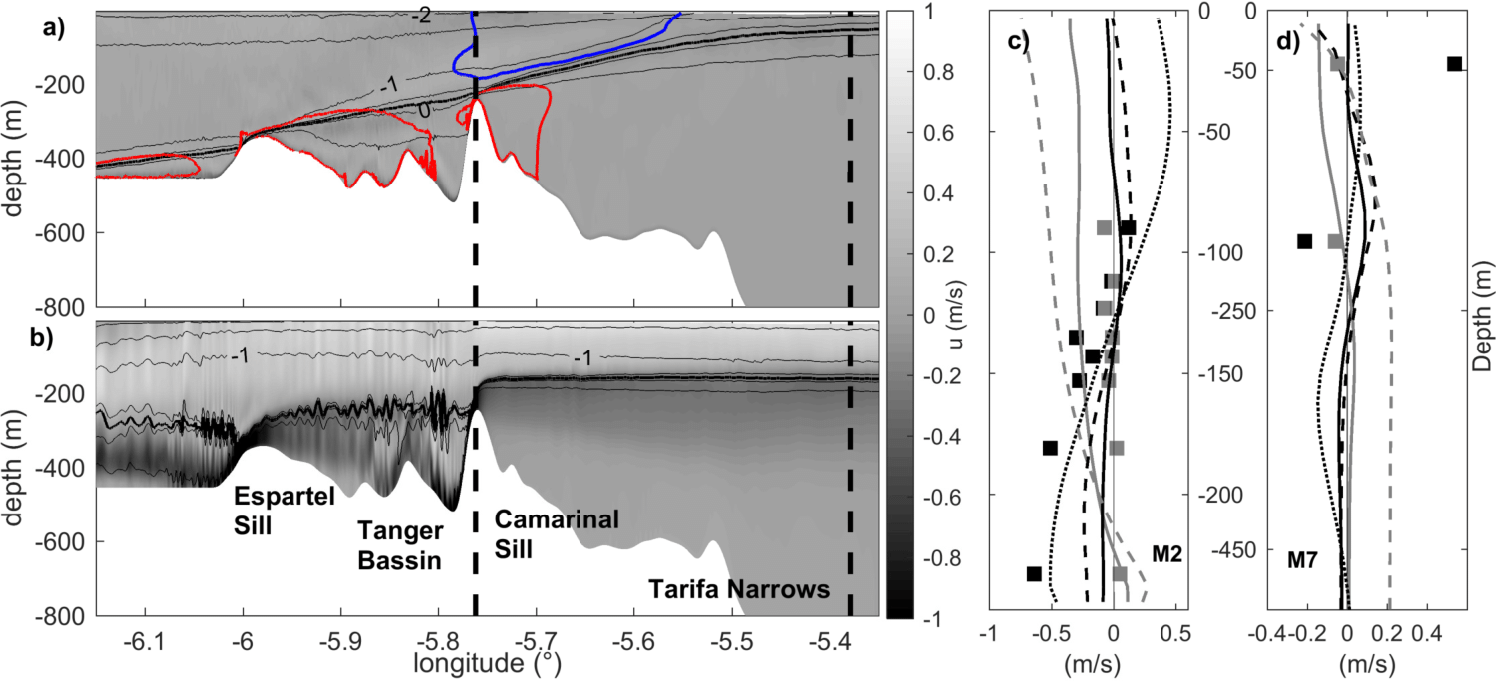
\includegraphics[width=\textwidth]{./GBR2D/figure4.png}
 \caption {a - b ) Longitudinal currents $u$ (greyscale) and isopycnals (thin black lines) of density anomaly between -2 kg m$^{-3}$ and 0.5 kg m$^{-3}$ with an interval of 0.5 kg m$^{-3}$ at t = 72 h at the end of the spin-up phase for \textbf{SimAllCor} (a) and \textbf{SimNoCor} (b). The bold line is for isopycnal $\rho' = -0.7 \ kg/m^3$. The vertical dashed lines indicate the location of the profiles given in c and d. Color contours in (a) indicate the values of transverse currents $v$. Inside the red contours $v \geq 0.5 \ m/s$, while inside the blue contours $v \leq -0.5 \ m/s$.  
  c - d ) 3T-averaged longitudinal currents (black) and transverse currents (grey) for \textbf{SimRef} (plain), \textbf{SimAllCor} (dashed) and \textbf{SimNoCor} (dotted). Observation of tidal-mean currents at stations M2 and M7 (Fig. \ref{Fig1}) from \citet{CW90} (squares).}
  \label{fig2}
\end{figure}

With no coastal boundaries to hinder the geostrophic adjustment within the strait, the initially longitudinal gravity current is almost completely converted into transverse geostrophic current with spurious (non physical) consequences on the slope of the isopycnals. Geostrophy enables a thermal-wind balance for the transverse $v$ component: 
\begin{equation}  
    \label{Thermal_wind}
    \displaystyle   
	\frac{\partial v}{\partial z}
    =-\frac{g}{\rho_0 f} \frac{\partial \rho}{\partial x}
\end{equation}
This is particularly apparent to the east of the CS in Figure \ref{fig2}.a where the pycnocline is located at the transition between positive and negative transverse velocities. As a consequence, the pycnocline slope is $\Delta z/\Delta x = 6.10^{-3}$ (Table \ref{tabdepth}) and the Atlantic water cannot spread further than the resulting surface front. In \textbf{SimRef}, the Coriolis force is introduced only after a 72-h-spin-up period leading to the state presented in Figure \ref{fig2}.b. In this case, the resulting slope and transverse velocity are smaller than in \textbf{SimAllCor}. %(figure \ref{fig_current}.c). 
The pycnocline in the eastern part of the domain is deeper whereas it is shallower in the western part. However, longitudinal currents remain weak. In contrast, in \textbf{SimNoCor} the thermal-wind balance is not allowed and, away from the sills, $\Delta z/\Delta x$ vanishes. In the longitudinal direction, the main balance is between the pressure force $(-1/\rho_0\  \partial p/\partial x)$ and the acceleration term. In this case, the shear of the longitudinal velocity is better represented at the two moorings. The larger transports in both layers indicate that a larger amount of Mediterranean water enters the Tangier basin than in \textbf{SimAllCor}. This is confirmed by the stratification (Figure \ref{fig2}.a and Table \ref{tabdepth}) since the pycnocline is shallower over the Espartel Sill (and deeper within the TN).

A perfect balance between the transports in the upper and lower layers is not achieved in any of these three numerical experiments. While there is no numerical challenge in achieving longer simulation, the fluxes of Mediterranean and Atlantic waters are not realistically specified to re-stratify properly the water column in these academic configurations. After the spin-up period, the intense tidal mixing and other dissipative processes may end up homogenizing the initial water masses. The gap between the transports in the upper and lower layers disappears as the depth-averaged absolute transports decrease. This process is faster in \textbf{SimNoCor} than in the other configurations in which the thermal-wind balance maintains the isopycnal slopes. In this case, the depth of the 37 psu-isohaline, taken as a moving average over one tidal period at x = $5.4^\circ$W, increases from 130 to 175 m in \textbf{SimNoCor} over three tidal periods (not shown). This impacts the large-amplitude internal waves propagation.

The difficulty to obtain both realistic ambient stratification and circulation is a limitation of the restriction to a 2D vertical section of the dynamical problem targeted. In the proposed implementation, an initial state is obtained by lock-exchange with a spin-up period of 72 h dedicated to the adjustment of the gravity current produced by the 'dam break'. For the remainder of this paper, the reference simulation (\textbf{SimRef}) is chosen as the simulation whose adjustment is made in a non-rotating framework. This initial state has a correct mean exchange but it is weakened as the tidal forcing is introduced and changes the stratification conditions.

To mitigate this problem, the rotation is restored at the end of the spin-up period: the geostrophic balance that ensues stabilizes the slopes of isopycnals by generating a transverse current. The mean exchange is nevertheless reduced but the stratification (i.e. both the slope of the isopycnals and the vertical density gradient) thus saved is crucial to the generation and propagation of the large-amplitude solitary waves. Furthermore, the small-scale processes discussed hereafter take place during the tidal cycle. At this time-scale, the barotropic exchange is dominated by the tidal currents, so that in the reference simulation, the amplitude of the baroclinic exchange is correct. Note that if rotation is activated from the beginning of the spin-up period (\textbf{SimAllCor}), it leads to unrealistically-large slopes of the isopycnals (see Table \ref{tabdepth}). 


%%%%%%%%%%%%%%%%%%%%%%%%%%%%%%%%%%%%%%%%%%%%%%%%%%%%%%%%%%%%%%%%%%%%%%%%%%%%%
\subsection{The Reference Simulation}
\label{sRef}
%%%%%%%%%%%%%%%%%%%%%%%%%%%%%%%%%%%%%%%%%%%%%%%%%%%%%%%%%%%%%%%%%%%%%%%%%%%%%

\indent The reference simulation presented previously is now evaluated thanks to the observational data from the Gibraltar Experiment \citep{FA1988}. We describe the hydraulic controls, the primary instabilities and the dynamics of the ISW in this reference simulation.

%----------------------------------------------------------------------------
\subsubsection{Comparison with \textit{in situ} Observations}
\label{refobs}
%----------------------------------------------------------------------------

\indent In the present section, observations from the Gibraltar Experiment \citep{FA1988} are investigated in order to evaluate the quality of the model solution obtained with the reference configuration \textbf{SimRef}.

The table \ref{tabdepth} presents the pycnocline depth and slope at different locations along the section for the three configurations and the observational data. The depth and slope for \textbf{SimAllCor} and \textbf{SimNoCor} are calculated after 72 h of simulation and correspond to the isopycnal surface $\rho'$= -0.7 kg/m$^3$ in figures \ref{fig2}.a-b, whereas for configuration \textbf{SimRef} the same isopycnal taken in a 3T-averaged stratification corresponding to Figure \ref{fig_fn_ref}. In \textbf{SimAllCor}, the isopycnals have a greater slope than the reported observations from Gibraltar Experiment (0.006 vs 0.003). In \textbf{SimNoCor}, there is no slope away from the sills, while as discussed before, the slope obtained in \textbf{SimRef} is small. The stratification in \textbf{SimRef} is close to that of \textbf{SimNoCor} in the eastern part with an isopycnal close to the horizontal. In the western part and over the CS, the pycnocline is shallower than in the other two simulations (Table \ref{tabdepth}).

In the following, we further investigate small-scale dynamical processes such as hydraulic jump and ISW propagation in configuration \textbf{SimRef}. This is also the baseline configuration used to perform all sensitivity tests presented hereafter.

%%%%%%%%%%%%
% Table 
%%%%%%%%%%%%
\begin{table}[!h]
 \caption{3T time-averaged transports (m$^2$/s) at CS, depth (m) and slope of the interface.}
 \centering
  %\begin{tabular}{|l|c|c||c|c|c||c|c|}
  \begin{tabular}{|p{0.1\linewidth}|p{0.1\linewidth}|p{0.1\linewidth}||p{0.1\linewidth}|p{0.1\linewidth}|p{0.1\linewidth}||p{0.09\linewidth}|p{0.09\linewidth}|}
 \hline
 &\multicolumn{2}{c||}{Transport (m$^2$/s)} & \multicolumn{3}{c||}{Pycnocline Depth (m)} & \multicolumn{2}{c|}{Pycnocline Slope}\\
  \hline
   &Upper  & Lower & ES & CS & TN& ES-CS & CS-TN\\
    &layer &layer &(5.91$^\circ$W)&(5.71$^\circ$W)&(5.52$^\circ$W)& & \\
   \hline
   \citet{FA1988} & / & / & 190  & 125 & 60 & 0.003 & 0.003\\
   \hline
   \textbf{SimAllCor} & -5 & -13 & 300 & 175 & 70 & 0.006 & 0.006\\
   \hline
   \textbf{SimNoCor} & 50 & -45 & 290  & 200 & 220& 0.005 & -0.001\\
   \hline
   \textbf{SimRef} & 0.7& -6 & 245 & 175 & 160 & 0.004 & 0.001\\
  \hline
 \end{tabular}
 \label{tabdepth}
\end{table}

%%%%%%%%%%%%%%%%%%%%%%%%%%%%%%%%%%%%%%%%%%%%%%%%%%%%%%%%%%%%%%%%%%%%%%%%%
\subsubsection{Tidal Currents \& Hydraulic Control.}
\label{tide_hyd}
%%%%%%%%%%%%%%%%%%%%%%%%%%%%%%%%%%%%%%%%%%%%%%%%%%%%%%%%%%%%%%%%%%%%%%%
\begin{figure}[!h]
\centering
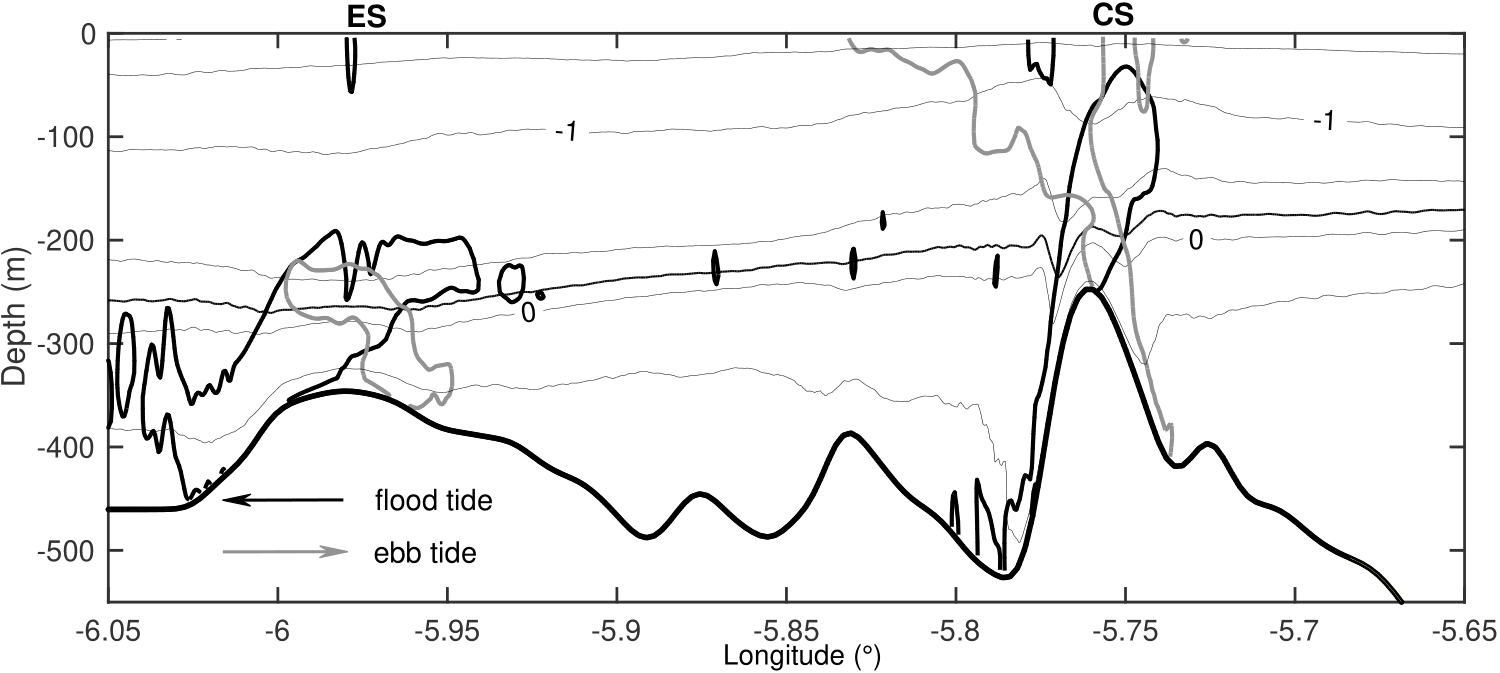
\includegraphics[width=1\linewidth]{./GBR2D/figure5.png}
\caption{ Isopycnal position averaged over a 3T time interval in \textbf{SimRef} (thin black lines are density anomaly contours between -1.5 kg m$^{-3}$ and 0.5 kg m$^{-3}$ with an interval of 0.5 kg m$^{-3}$;  
%the bold line shows $\rho'$ = -0.7 kg/m$^3$). 
Thick black (grey) contours indicate critical Froud number $F=1$ during flood (ebb) tide, inside which the flow is supercritical.}
\label{fig_fn_ref}
\end{figure}


In the present study, the Froude number ($F$) is simply defined at each grid point as the ratio between the local longitudinal velocity $u$ and the theoretical speed $c_1$ of the first internal wave mode, computed with the modal decomposition for each point of the x-axis (see \ref{app_Froude} for details).

For single-layer flows, hydraulic control occurs in the region of transition between subcritical and supercritical flows. In this region, the condition $F>1$ is met over the whole water column. For multi-layer flows, the Froude number condition may be satisfied in a few layers only. In this case, the layers where the flow becomes supercritical are considered as "hydraulically controlled".

Three areas of potential hydraulic control in Gibraltar Strait are identified from previous studies: the CS, the ES and the narrowest part of the TN (near 5.5$^\circ$W longitude in figure \ref{Fig1}). \citet{FA1988} found persistent controls for first internal wave mode at the ES, the CS and the TN. \citet{Sannino2009b} found only ephemeral appearances of such controls, except at the ES where it is permanent. The discrepancy is likely lying in the definition and the estimation of the composite Froude number.

Figure \ref{fig_fn_ref} shows the regions where the flow is critical. Closed contours indicate the locations of critical Froude number ($F=1$), inside which the flow is supercritical. The longitudinal velocity fields ($u$) used to estimate F are taken at maximum outflow (grey) at $t = 7.5\ T$ and maximum inflow (black) at $t = 8\ T$. The internal waves phase speed $c_1$ is computed from the 3T-time-averaged stratification represented in Figure \ref{fig_fn_ref}. No control of the first mode is ever seen in TN : this is a consequence of the 2D simplification which excludes the representation of the tidal flow intensification by the narrowing of the strait at TN. On the other hand, hydraulic control is expected at both sills. The location where it should occur alternate between the eastern (during ebb) and western (during flood) sides of the sills, with a return to subcritical flow when tidal current slackens. The Froude number easily goes beyond 2 in the Mediterranean outflow at CS, where the flow is supercritical through most of the water column, except sometime at the surface. At ES, the lower layer may become supercritical with Froude number that never exceeds 1.5. The lack of persistent control at ES may be a consequence of the crudely imposed stratification.

%-----------------------------------------------------------------
\subsubsection{Primary Instabilities in the Hydraulic Jump Area}
\label{section_insta2D}
%-------------------------------------------------------------------

\begin{figure}[!h]
\centering
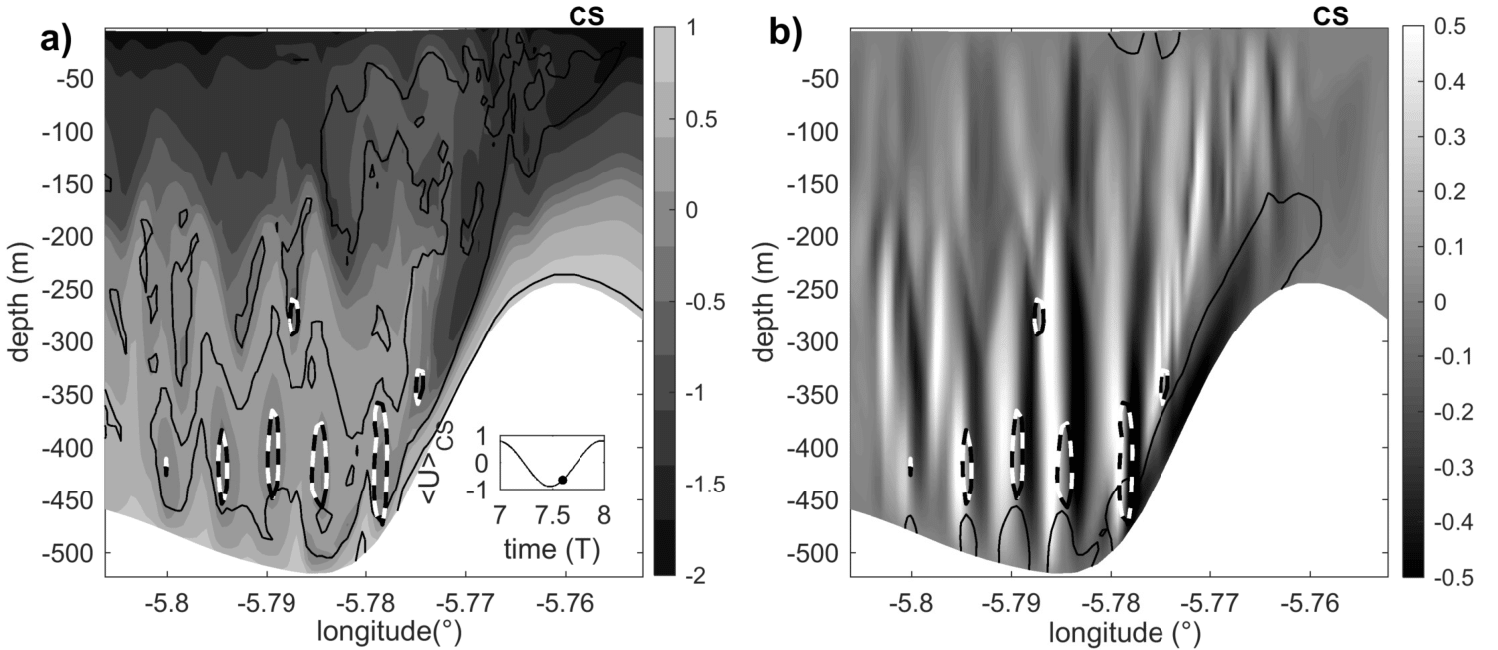
\includegraphics[width=1\linewidth]{./GBR2D/figure6.png}
	\caption{a) Density anomaly (greyscale ; $kg/m^3$) in the lee side of Camarinal Sill in \textbf{SimRef} at t = 7.56 T. Black contours indicate the location where the Richardson number is  0.25. b) Vertical velocity (greyscale ; $m/s$) in the lee side of Camarinal Sill in \textbf{SimRef} at t = 7.56 T. The black contour indicates the location where the Froude number is 1. a) and b) The black and white contour represents $OW=-4*10^{-4}\ s^{-2} $.} 
\label{RH_CS}
\end{figure}

One manifestation of the hydraulic control is the formation of hydraulic jumps in specific regions where the flow transitions from supercritical to subcritical. This is a complex area with steep slopes and high shears where flow-topography interaction can generate small-scale coherent structures. The largest ones are resolved in \textbf{SimRef} and are characterised here with various methods. First, the Okubo-Weiss parameter (\ref{annexeOW}) is computed to investigate the presence of new 'coherent structures' in the hydraulic jump area. Their dynamics are further investigated using Empirical Orthogonal Functions (EOFs) computed with a Singular Value Decomposition (SVD). Their typical length and velocity scales are finally compared with the expected analytical values of shear instabilities and lee waves.

The dynamics of the CS hydraulic jump are illustrated in Figure \ref{RH_CS}, in which the density field (Fig. \ref{RH_CS}.a) and the vertical velocity field (Fig. \ref{RH_CS}.b) over the western slope of the CS are represented during flood. Several flow parameters were also computed and are depicted in Figure \ref{RH_CS}.a and b. These parameters are :

\begin{enumerate}

\item
The Froude number defined in \ref{app_Froude}. The contours of critical Froude number $F=1$ are shown in Figure \ref{RH_CS}.b, inside which the flow is supercritical.

\item
The Richardson gradient number defined as $Ri =  N^2 / \left({\partial u}/{\partial z}\right)^2$, with $N$ the Brunt-V\"ais\"al\"a frequency defined in Eq.\ref{eqN}. Contours of $Ri = 0.25$ are depicted in Figure \ref{RH_CS}.a, as $Ri<0.25$ is a required condition for the development of shear instabilities.

\begin{equation}
N=\sqrt{ - \frac{g}{\rho_0} \frac{\partial \rho}{\partial z}}
\label{eqN}
\end{equation}

\item
The Okubo-Weiss parameter defined in \ref{annexeOW}. Negative values of OW indicate vortical circulation, and so contours of $OW = -4*10^{-4}\ s^{-2}$ are shown in both Figure \ref{RH_CS}.a and b. 

\end{enumerate}

In Figure \ref{RH_CS}.b, the supercritical flow region (F $>$ 1)  follows the slope of the sill where the velocity in the Mediterranean outflow is larger than 2 m/s (see the contour F = 1 running approximately parallel to isopycnals between 5.76$^\circ$W and 5.77$^\circ$W). At 5.77$^\circ$W, the density field in Figure \ref{RH_CS}.a shows a sharp transition (e.g., isopycnal $\rho'=-0.5kg/m^3$ rises from 350 to 225 m depth), and forms a wedge-shaped region over the supercritical Mediterranean outflow. This is the signature of an internal hydraulic jump. 

Downstream of the hydraulic jump, several small-scale structures are visible. Figure \ref{RH_CS}.a shows patches of lighter water (billows) associated with areas of negative OW values at a depth of 400 m, and large-amplitude disturbances of isopycnals at 150 m. Negative OW values are also located at troughs and can reach $OW=-4*10^{-4} s^{-2} $. Both types of structures are propagating westward and are quite probably shed from the internal hydraulic jump at the tip of the wedge-shaped region at 5.773$^\circ$W, with the size of billows growing rapidly as they travel down-slope. In the potential generation area, Richardson number values are less than 0.25, indicating favorable conditions for generation of primary shear instabilities. 

Further identification of the simulated new features of Figure \ref{RH_CS} is achieved by proceeding with a complex singular value decomposition (SVD) \citep{Pairaud2005} of the velocity field $(w+iu)$ in the water column between 5.795$^\circ$W and 5.78$^\circ$W longitude, during outflow conditions. This region is highlighted in Figure \ref{eof_insta}.a, in which the time mean field of longitudinal velocity $u$ is presented, showing the intense outflow below layers of lesser velocities. The mean density field and location of $Ri\ <\ 0.25$ are also indicated, the former showing a homogeneous area between 50-150 m above the seafloor. The SVD gives a first singular vector responsible for $28\ \%$ of the total variance corresponding to the evolution of the barotropic forcing (not shown). The remaining singular eigenvectors have lesser corresponding variance and show smaller structures with high-frequency variations in the singular right eigenvector. Two consecutive singular vectors often have very close eigenvalues and temporal variations.

\begin{figure}[!h]
\centering
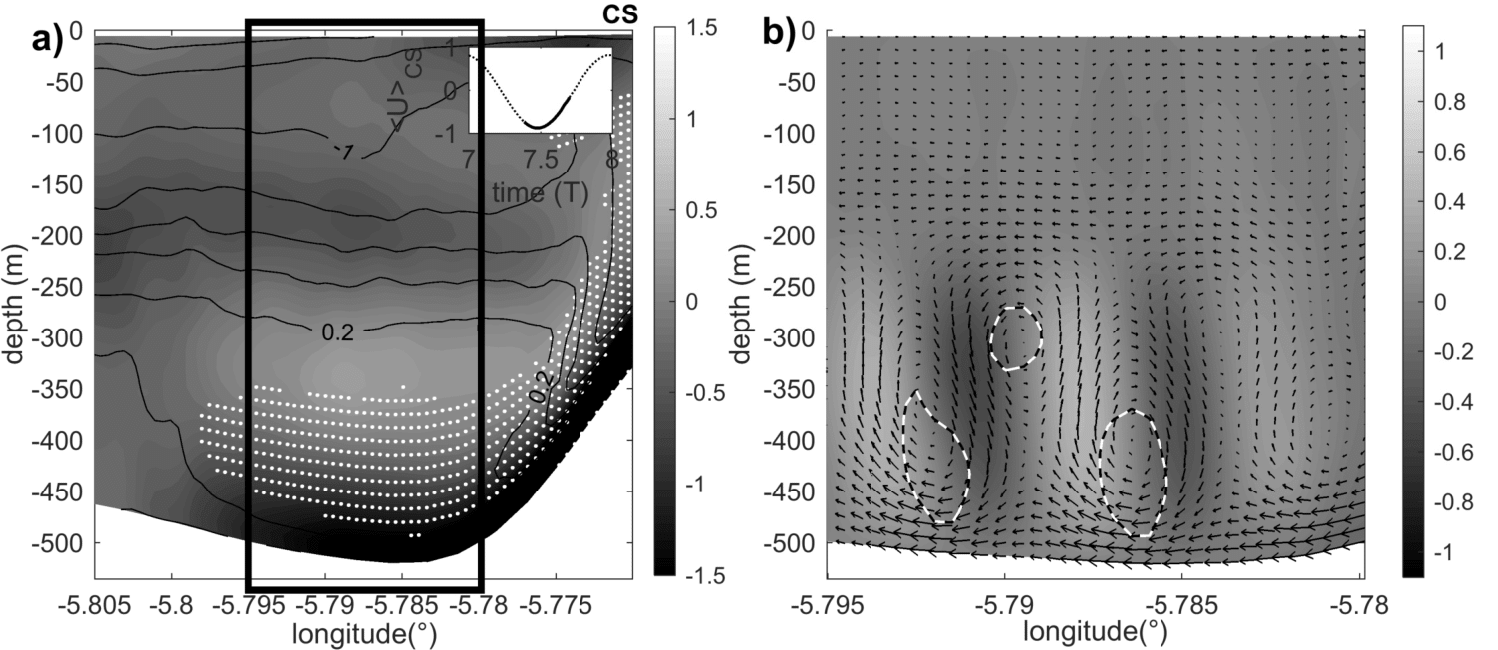
\includegraphics[width=1\linewidth]{./GBR2D/figure7.png}
 \caption {a) Mean field of longitudinal velocity $u$ (m/s) ; greyscale) and isopycnals (black lines, density anomaly between -1.6 kg m$^{-3}$ and 0.5 kg m$^{-3}$ with an interval of 0.3 kg m$^{-3}$ ) with location of Ri$<$0.25 (white dots). b) Vertical velocity $w$ (greyscale ; m/s) and velocity vectors of the superposition of the second and third singular vectors of the SVD decomposition added to the mean velocity field of (a). Black and white contours are OW=$ -1.5*10^{-4}\ s^{-2}$}
 \label{eof_insta}
\end{figure}

Figure \ref{eof_insta}.b shows the reconstructed field of the combination of the second and third singular vectors (respectively responsible for $13\ \%$ and $11\ \%$ of total variance) added to the mean field shown in Figure \ref{eof_insta}.a. The Okubo-Weiss parameter is again computed for the resulting velocity field, which shows two rows of y-axis vortices centered at z = -300 m (anti clockwise) and -400 m (clockwise). The upper row of vortices appears to generate the observed interface oscillations.

Based on OW$=$0 contours, the lower clockwise vortices have an estimated horizontal scale of 200 m and a vertical scale of 150 m, corresponding to horizontal and vertical wavenumbers 3.10$^{-2}$ and 4.10$^{-2}$ m$^{-1}$ respectively. Their propagation speed can be estimated as -0.7 m/s by following the center of the billows defined by areas of negative OW values. The distance between the centers of two consecutive vortices is L = 530 m. The centers of the upper anti-clockwise and lower clockwise vortices are shifted along flow by L/2, so that the extrema of their respective vertical velocities are aligned vertically. It seems that a transfer of momentum occurs between the two rows of vortices in a way reminiscent of the Vallis model of edge waves in a stratified region of a shear flow (pp 254-258 in \citet{vallis_atmospheric_2006}). 

The length scales deduced from this SVD analysis can now be compared with expected scales from simple analytical models for shear instabilities and internal waves based on the general characteristics of the flow on the western slope of Camarinal.

Shear flow instability in a two-layer system of infinite depth results in a mixed interface of vertical extent $\Delta H$ expressed by equation 14.6 of \citet{Cushman-RoisinBenoit2011} :
%
\begin{equation}
\Delta H \approx \frac{1}{k_{min}} = \frac{\rho_0 (u_1 - u_2)^2}{2(\rho_2-\rho_1)g}
\end{equation}
%
with $k_{min}$ the wave-number of the most unstable mode in this system, taken as the scale of the primary instability that will develop. In the generation area of CS, $(u_1-u_2)$ is in the range of 1.2 to 2 m/s and $(\rho_2-\rho_1)$ is in the range of 1.2 to 1.7 kg/m$^3$. Additional values are $\rho_0$ = 1033.7 kg/m$^3$ and g = 9.81 m$^2$/s. This gives a range of vertical scales between 44 m and 183 m and $k_{min}$ between 2.10$^{-2}\ m^{-1}$ and 5.10$^{-3}\ m^{-1}$. The scales of the simulated lower row of vortices are in the upper part of this range.

Lee waves are another candidate for small-scale transient flow and the interfacial oscillations observed in our solutions. Their generation over topography is expected when tidal excursion is larger that the topographic length scale $1/k_b$, i.e, $k_b u_0/\omega > 1$ \citep{StLaurent2002}. The slopes of Camarinal Sill are not symmetrical, as can be seen for example in Figure \ref{fig2}. On the western side of the sill, the depth increases from 250 m (at 5.76$^\circ$W) to 510 m (at 5.78$^\circ$W) over only 1.8 km, whereas on the eastern side it increases from 250 m to 620 m (at 5.65$^\circ$W) over 9.4 km. $k_b$ is thus chosen in a range between $3.10^{-3}\ m^{-1}$ and $6.10^{-4}\ m^{-1}$. $u_0=0.4\ m/s$ is the amplitude of the barotropic tidal current away from the sill. In these conditions, the ratio $k_b u_0/\omega$ ranges between 1.7 (over the west slope) and 8.9 (over the east slope). Based on this, we cannot rule out the possibility that lee waves are generated over the CS.

If the simulated small-scale structures would originate from lee waves, their phase speed would be comparable to a mode-1 internal gravity waves. This can be estimated using the same method as in \ref{app_Froude} for the average stratification presented in Figure \ref{eof_insta}.a. It yields a value of 1.4 m/s in the area down-flow of the hydraulic jump, which is twice the estimated propagation speed of both rows of simulated structures. Therefore, even though lee-wave generation is theoretically possible, the interfacial oscillations observed in the simulation appear more consistent with the stirring effect of the bottom coherent vortices, whose scales fall within the range of expected values for KH instability.

We conclude that coherent structures are clearly identified in our simulations. They are generated in an area of potentially unstable shear $(Ri\ <\ 0.25)$ and are associated with billows of lighter mixed fluid. The deeper row of vortices can reasonably be interpreted as Kelvin-Helmholtz primary instabilities. Their downstream behaviour further corresponds to a 2D pairing of two consecutive Kelvin-Helmholtz billows. These billows are advected in a region of westward flow between the Mediterranean vein and  Atlantic waters up until 5.8$^\circ$W. At this location, advection is reduced as the lower layer decelerates and the billows are uplifted in a flow recirculation and mixed in the pycnocline.
These small-scale features appear in the simulation for as long as the hydraulic jump is present, injecting water from the pycnocline in the outflow and vigorously mixing the Atlantic and Mediterranean waters until the tidal currents weaken sufficiently for the flow to become subcritical. 

 However, the dynamics simulated in a 2D vertical section with no transverse flow and no transverse instability may differ from the real ocean. In a fully 3D configuration, primary Kelvin-Helmholtz instabilities should decay faster as secondary Kelvin-Helmholtz instabilities develop along the transverse rotation axis of the primary billows. This is precluded in the present 2D configuration, even with enhanced resolution, as only y-axis billows can occur.

\citet{wesson_1994} observed billow structures in the area of CS with an extension of several tens of meters. This length scale is much smaller than the one simulated in the present numerical configuration. However, these observations were made in shallower regions, i.e. probably closer to the generation area: larger billows more in line with those simulated in the present study could thus develop downstream. Further observations on site are needed, although short length-scales and fast propagation speed would require adapted measurement strategies.

%------------------------------------
\subsubsection{Internal Tide Dynamics}
\label{sisw}
%------------------------------------

\begin{figure}[!h]
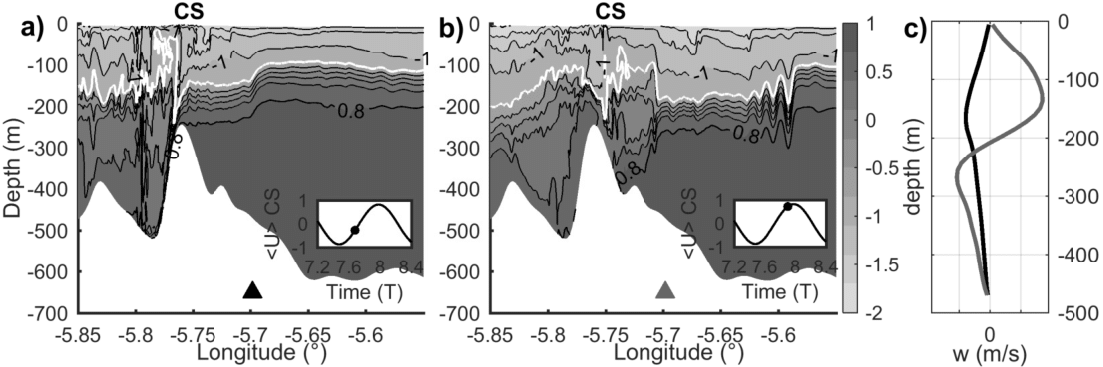
\includegraphics[width=\textwidth]{./GBR2D/figure8.png}
  \caption{Density anomaly fields ($\rho$ ; $kg/m^3$) of \textbf{SimRef} zoomed over CS at t = 7.7 T (a) and t = 7.9 T (b). The position of $\rho'\ =-0.7\ kg/m^3$ isopycnal is shown in white. c) Profiles of vertical velocity at the position marked by a triangle in (a)-black and (b)-grey.}
  \label{fig_gen_CS}
  \end{figure}
  
\begin{figure}[!t]
\centering
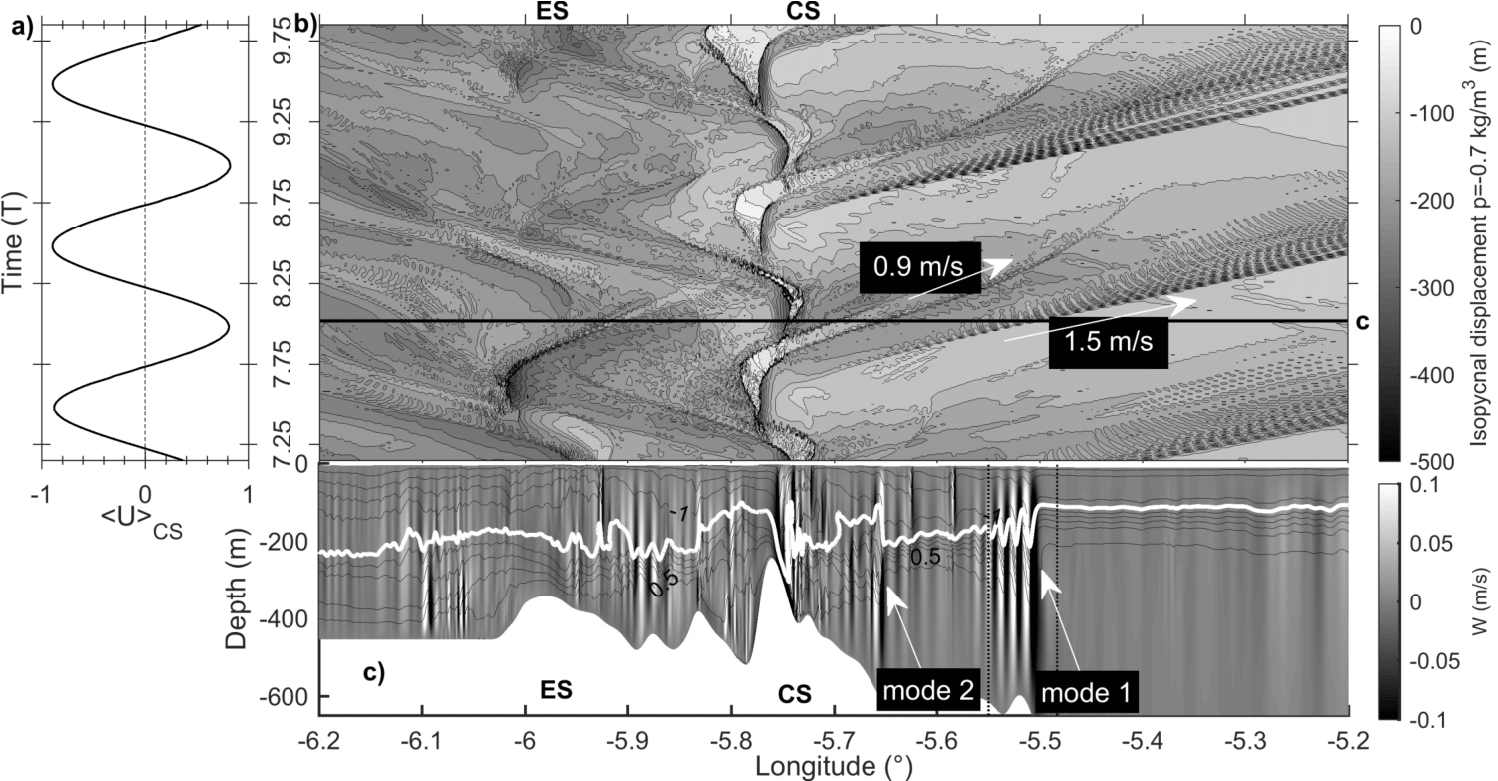
\includegraphics[width=1\linewidth]{./GBR2D/figure9.png}
 \caption {(a) Depth-averaged currents over CS. (b) Space-time diagram of the vertical displacement of isopycnal $\rho' = -0.7\ kg/m^3$ of \textbf{SimRef} ($\Delta z = 50\ m$ between two contours). The black line indicates the time used in the bottom panel. (c) vertical velocity field (greyscale) and isopycnals (black lines ; density anomaly between -1.9 kg m$^{-3}$ and 0.5 kg m$^{-3}$ with an interval of 0.3 kg m$^{-3}$ ) at the time indicated in panel (b). In white is the isopycnal $\rho' = -0.7\ kg/m^3 $.}
 \label{hov_ref}
\end{figure}

In \textbf{SimRef}, two main types of large amplitude wave propagating eastward can be observed. Both of them are generated at CS while tidal currents reverse from westward to eastward. This is illustrated in Figure \ref{fig_gen_CS}.a-b. First, a mode-1 wave appears as a bore over the sill's crest approximately 2.25 hours after the westward flow peaks. 
In Figure \ref{fig_gen_CS}.a, it has propagated over the eastern slope of the sill's crest and is now at 5.7$^\circ$W longitude: the corresponding profile in Figure \ref{fig_gen_CS}.c has only one maximum as expected for a mode-1 internal wave. This wave rapidly steepens while a hydraulic control is maintained on the western side of the sill with lower values of the Froude number. One hour and 15 minutes later, the flow becomes subcritical and a large-amplitude mode-2 wave crosses the sill. 
In Figure \ref{fig_gen_CS}.b, this new wave is propagating over the eastern slope of the sill; its vertical velocity profile is presented in Figure \ref{fig_gen_CS}.c. It exhibits two maxima of opposite signs and a zero-crossing at the pycnocline's depth as expected for a mode-2 internal wave. Additionally, it can be seen in this figure that the bore-like wave has evolved into a train of internal solitary waves, whose propagation is discussed bellow. 

The propagation of internal waves can be characterized by plotting a space-time evolution of a particular isopycnal. In Figure \ref{hov_ref}.b, the depth evolution of the $-0.7\  kg/m^3$ isopycnal is represented (also in a white contour in Fig. \ref{fig_gen_CS}). Regions of sharp horizontal density gradients can be identified periodically in the region of the CS next to 5.76$^\circ$W longitude. They correspond to the generation of hydraulic jumps. The propagation of internal waves are identified by the tilt of isolines, whose slopes provide an estimate of wave propagation speed. There are differences from one tidal cycle to the next because mixing progressively changes the background stratification in the domain. In the following, we focus on the tidal cycle $t\ =\ 7.5\ T\ -\ 8.5\ T$ (second cycle after the end of the spin-up phase), for which the three-tidal-cycle averaged velocity shear and stratification are shown in Figures \ref{fig2} and \ref{fig_fn_ref}.

The mode-1 bore of Figure \ref{fig_gen_CS}.a propagates down-slope of the CS into the TN, where it experiences a transition into a train of solitary waves moving at a speed of 1.5 m/s. In Figure \ref{hov_ref}.c, such a train made of four mode-1 waves can be seen at 5.5$^\circ$W longitude. The amplitude of the first wave reaches 100 m. The solitons train amplitude momentarily increases and exceeds 150 m as it propagates over the slope near 5.5$^\circ$W longitude in the TN (still during ebb tide). From then on, the wave amplitude decreases as it propagates towards the deeper region. Meanwhile the dispersion increases the number of waves as well as their wavelength as noticed in the space-time diagram which shows the envelop of the train of solitons expanding while it propagates eastward. The dispersion as simulated in CROCO is compared with the Korteweig deVries model in \ref{KdVpart}.

Similarly, the mode-2 wave shown in Figure \ref{fig_gen_CS}.b propagates through the shallowest part of the TN at a speed of 0.9 m/s as a new hydraulic jump is being generated over the eastern slope of CS. It is located at 5.65$^\circ$W longitude in Figure \ref{hov_ref}.c, with an amplitude of approximately 100 m. The propagation speed of this mode-2 internal wave subsequently decreases when it reaches the deepest part of the domain while simultaneously the tidal phase shifts to flood. The amplitude of these waves is simultaneously strongly reduced.

The signatures of other large-amplitude internal waves can be seen propagating to the west of the CS in Figure \ref{hov_ref}.b. They are mode-1 and mode-2 internal waves with amplitude in the tens of meters, i.e. smaller than the eastward propagating wave. They are generated when tidal currents switch from eastward to westward in the same fashion as previously described for the wave train produced east of the CS (as tidal currents reverse from westward to eastward).

As discussed in Section \ref{tide_hyd}, a hydraulic control also occurs at the ES. Figure \ref{hov_ref}.b shows the same variations of  isopycnal depth in this area as near the CS during the tidal cycle $t\ \in [\ 7.5\ T,\ 8.5\ T\ ]$, but not on the following cycle anymore. In the latter case, the computed Froude number does not exceed 0.7, as opposed to previous cycles ($t\ \in[\ 6.5\ T,\ 7.5\ T\ ]$ and $t\ \in[\ 7.5\ T,\ 8.5\ T\ ]$) or later ones ($t\ \in[\ 9.5\ T,\ 10.5\ T\ ]$ and  $t\ \in[\ 10.5\ T,\ 11.5\ T\ ]$). In these cases, the variations are similar and hydraulic control occurs at ES. The sequence is as in CS, with a hydraulic control briefly lost at the barotropic flow reversal. Then internal mode-1 waves of 50-m amplitude at a depth of 300 m are released and propagate toward the CS. In Figure \ref{hov_ref}.c, a mode-1 wave can be found at 5.87$^\circ$W. These waves dissipate in the area near the sill as the absolute value of the barotropic current decreases.

In Figure \ref{hov_ref}.c, two vertical lines are drawn in the TN. They refer to measurements made by \citet{FA1988}: the lines indicate the first two baroclinic modes locations three and a half hours after high tide. The right-hand vertical line corresponds to a mode-1 wave and is in agreement with the simulation. However, in \textbf{SimRef}, the distance between the two modes is twice as large as in the observations. Based on observed wave arrivals at various stations, \citet{FA1988} estimated the propagation speed of both mode-1 and mode-2 waves at about 1 to 2.5 m/s for mode 1 and 1 to 1.5 m/s for mode 2. The wave train they observed contained two to three large-amplitude waves, the first one having an amplitude of 100 m. Additional observations by \citet{SG2008} in the TN region give a propagation speed for mode-1 waves ranging in 1.2 m/s and 2 m/s with a large variation in the velocity of two consecutive wave trains due to the weight of the tidal diurnal inequality (K1 and O1).

The mode-1 dynamics simulated in \textbf{SimRef} are consistent with these observations reported by \citet{FA1988} in terms of propagation speed and longitudinal position. However, the simulated mode-2 wave seems too slow and its amplitude too large. Its slower propagation might be due to an underestimation of the barotropic flow that carries the mode-2 within the TN as our 2D vertical approach does not catch well the tunneling effects of this narrowing. This would not affect the mode-1 wave as much, because its linear propagation speed is more intense and the barotropic current advection becomes comparatively small.

The brief hydraulic control loss observed when the tidal currents reverse does not reflect the quasi-permanent control thought to be taking place at ES. In this case, no internal waves packet can be emitted from the ES.


%%%%%%%%%%%%%%%%%%%%%%%%%%%%%%%%%%%%%%%%%%%%%%%%%%%%%%%%%%%%%%%%%%%%%%%%%%%%%
\subsection{Sensitivity Testing}
%%%%%%%%%%%%%%%%%%%%%%%%%%%%%%%%%%%%%%%%%%%%%%%%%%%%%%%%%%%%%%%%%%%%%%%%%%%%%

The reference configuration presented in the previous section is based on several physical and numerical choices which are now investigated ; mostly the impact of the forcing amplitude, momentum balance (hydrostatic approximation) and numerical parameters (spatial resolution, advection schemes). 

%----------------------------------------------------------------------------
\subsubsection{Tidal regime}
\label{TestAmp}
%----------------------------------------------------------------------------

An additional simulation, \textbf{SimS}, is first performed similarly to \textbf{SimRef} changing only the tidal forcing amplitude. The imposed tidal current amplitude at the western boundary is now increased up to 0.6 m/s, so that it reaches 1.3 m/s over the CS. This corresponds to a spring-tide regime.

Figure \ref{fig_cv_spring} presents a comparison between \textbf{SimS} and \textbf{SimRef}. In Figure \ref{fig_cv_spring}.a, the contours of supercritical regions ($F\ >\ 1$) show the the CS hydraulic jump extends further east in \textbf{SimS}. As a result, a mode-1 disturbance (denoted "a" in Figure \ref{fig_cv_spring}.a) is trapped at 5.725$^\circ$W longitude. It propagates eastward when the flow becomes subcritical but the faster bore that is crossing the CS can rapidly catch it up. The outflowing Mediterranean water vein on the westward side of the sill is also thicker in \textbf{SimS} and so is the supercritical area. In addition, a new supercritical region appears on the western slope of a secondary relief at 5.83$^\circ$W longitude (denoted "b" in Figure \ref{fig_cv_spring}.a) with trailing lee waves.

the figure \ref{fig_cv_spring}.b shows an eastward propagating mode-1 solitons packet. Since the initial stratifications are similar, linear phase velocities are the same in \textbf{SimRef} and \textbf{SimS} at the begining. The amplitude of the first trough of the train is 50-m larger in \textbf{SimS} than in \textbf{SimRef}. This should result in increased propagation speed of the solitons in \textbf{SimS}, in contradiction with a slower propagation seen in Figure \ref{fig_cv_spring}.b. It can be explained by the stronger tidal currents advection in the opposite direction in \textbf{SimS}. A mode-2 wave is also generated in both \textbf{SimS} and \textbf{SimRef}, but is only visible in \textbf{SimRef} in Figure \ref{fig_cv_spring}.b as it quickly dissipates in \textbf{SimS} due to stronger tidal currents.
Consistent with our results, \citet{FA1988} show that the ISW amplitude increases with the tidal current during the spring-tide / neap-tide cycle. In addition,  two concomitant hydraulic jumps were observed in the strait during spring tide (\citep{SG2011}): they exhibit a transverse asymmetry, as the second jump only appears in the northern part of the strait. This could not be confirmed in the present 2D configuration.

\begin{figure}[!h]
  \centering
  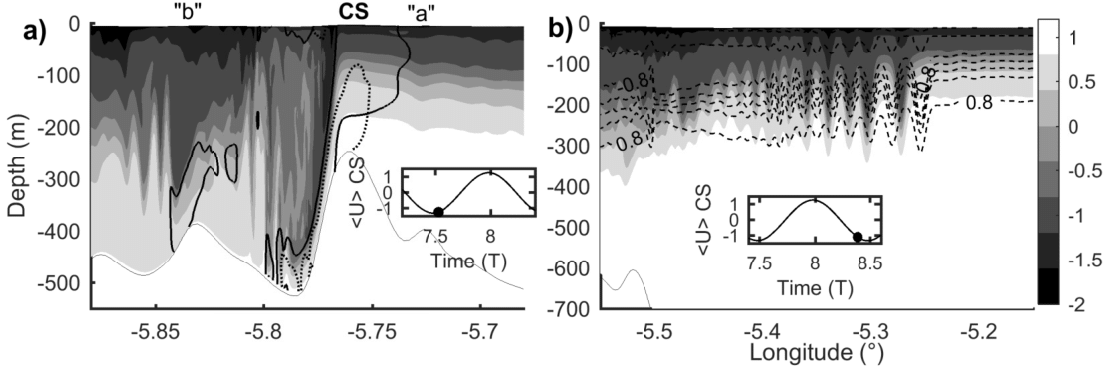
\includegraphics[width=1\textwidth]{./GBR2D/figure10.png}
  \caption{Comparison of experiments \textbf{SimS} and \textbf{SimRef} showing the effect of tidal amplitude on the generation of solitary waves. a) Relative density ($kg/m^3$) in \textbf{SimS} during a hydraulic jump ($t = 7.5\ T$) at Camarinal Sill. Regions where $F\ >\ 1$ are indicated for both \textbf{SimS} (bold lines) and \textbf{SimRef} (dashed lines). New features appear with stronger tides: a mode-1 disturbance "a" trapped upstream of the CS; an additional supercritical area ($F\ >\ 1$) noted "b" in the bottom layer of a secondary relief. b) Relative density in \textbf{SimS} (greyscale) and \textbf{SimRef} (dashed lines) at $t = 8.5\ T$, showing the tidal amplitude effect on eastward propagating solitary waves generated at CS.}
  \label{fig_cv_spring}
\end{figure}


%------------------------------------------------------------------
\subsubsection{Nonhydrostatic Balance and Numerical Factors}
\label{TestNum}
%------------------------------------------------------------------
The consequences of several numerical choices are now investigated by running five additional simulations whose differences with \textbf{SimRef} are laid out in Table \ref{tab_sensnum}. In particular, the sensitivity to both vertical and horizontal resolution is targeted. A hydrostatic kernel and a WENO5-Z advection scheme for momentum \citet{Borges2008} are also tested and compared with \textbf{SimRef}. We focus on the impact of these modifications on two types of small-scale processes studied in the previous sections: the primary (KH) instability generation in the hydraulic jump at the CS, and the eastward propagating solitary waves generated at the same place. 

\begin{table}[!h]
\caption{Parameters of numerical sensitivity experiments. If not explicitly indicated, $t_s$ and $t_f$ are the same as in Table \ref{tabsimref}.}
 \centering
  \begin{tabular}{|c|l|}
 \hline
  \textbf{SimH}& Hydrostatic equations ($t_s=0.5s$ ~ $t_f=0.25s$)\\
  \hline
  \textbf{SimW}& WENO5-Z momentum advection scheme\\
  \hline
  \textbf{SimV}& 80 $\sigma$-levels\\
  \hline
  \textbf{SimL}& 220-m horizontal resolution ($t_s=4s$ ~ $t_f=0.5s$)\\
  \hline
  \textbf{SimLH}& 220-m horizontal resolution with hydrostatic equations ($t_s=2s$ ~ $t_f=1s$)\\
  \hline
 \end{tabular}
	\label{tab_sensnum}
\end{table}

%-------------------------------------------------
\paragraph{Hydraulic Jump and Instabilities}
%-------------------------------------------------

\begin{figure}[!h]
\centering
  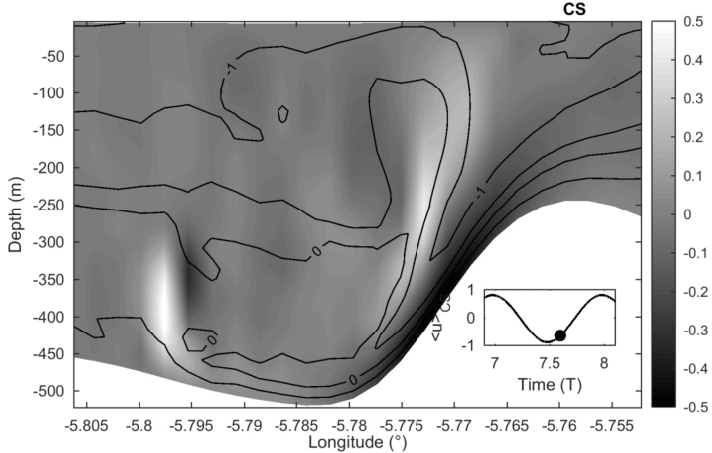
\includegraphics[width=0.7\textwidth]{./GBR2D/figure11.png}
  \caption {Vertical velocity (greyscale ; $m/s$ ) and isopycnals (black lines ; density anomaly between -1.5 kg m$^{-3}$ and 0.5 kg m$^{-3}$ with an interval of 0.5 kg m$^{-3}$ ) in \textbf{SimLH}.}
	\label{fig_sensnum1}
\end{figure}

Hydraulic controls (Section \ref{tide_hyd}) occur in all simulations, as revealed by systematic estimations of the Froude numbers. Low Richardson numbers ($<0.25$) are also diagnosed for all simulations over at least part of the CS western slope during flood. However, the features that have been identified as KH instabilities in Section \ref{section_insta2D} do not appear in all simulations. They are absent in the simulations performed in the hydrostatic framework and/or with low horizontal resolution (\textbf{SimL}, \textbf{SimLH} and \textbf{SimH}). Weak horizontal vorticity tilting under the hydrostatic assumption prevents such instabilities to develop. Instead, a smooth, large recirculation  appears west of the CS (Figure \ref{fig_sensnum1} for \textbf{SimLH}).

In the remaining sensitivity experiments (\textbf{SimV} and \textbf{SimW}), KH instabilities are generated at the edge of the hydraulic jump and their dynamics is overall similar to the one described in Section \ref{section_insta2D} for \textbf{SimRef}: pairing of KH billows can occur whereas anti-clockwise vortices induce oscillations of the interface. 
Fine resolution (a few tens of meters in the present region) and non-hydrostatic equations are both required to explicitly simulate the turbulent cascade onset with KH instabilities between Mediterranean and Atlantic flows. 

Interestingly enough, a comparison of Figures \ref{RH_CS} (nonhydrostatic configuration) and \ref{fig_sensnum1} (hydrostatic configuration) shows that the fine-scale solution is largely filtered out by the hydrostatic assumption. Without dedicated observations in the area, it remains difficult to conclude that \textbf{SimRef} is more realistic, although low Richardson numbers in this region lead us to expect KH instability.

\paragraph{Large Internal Waves}
\begin{figure}[!h]
  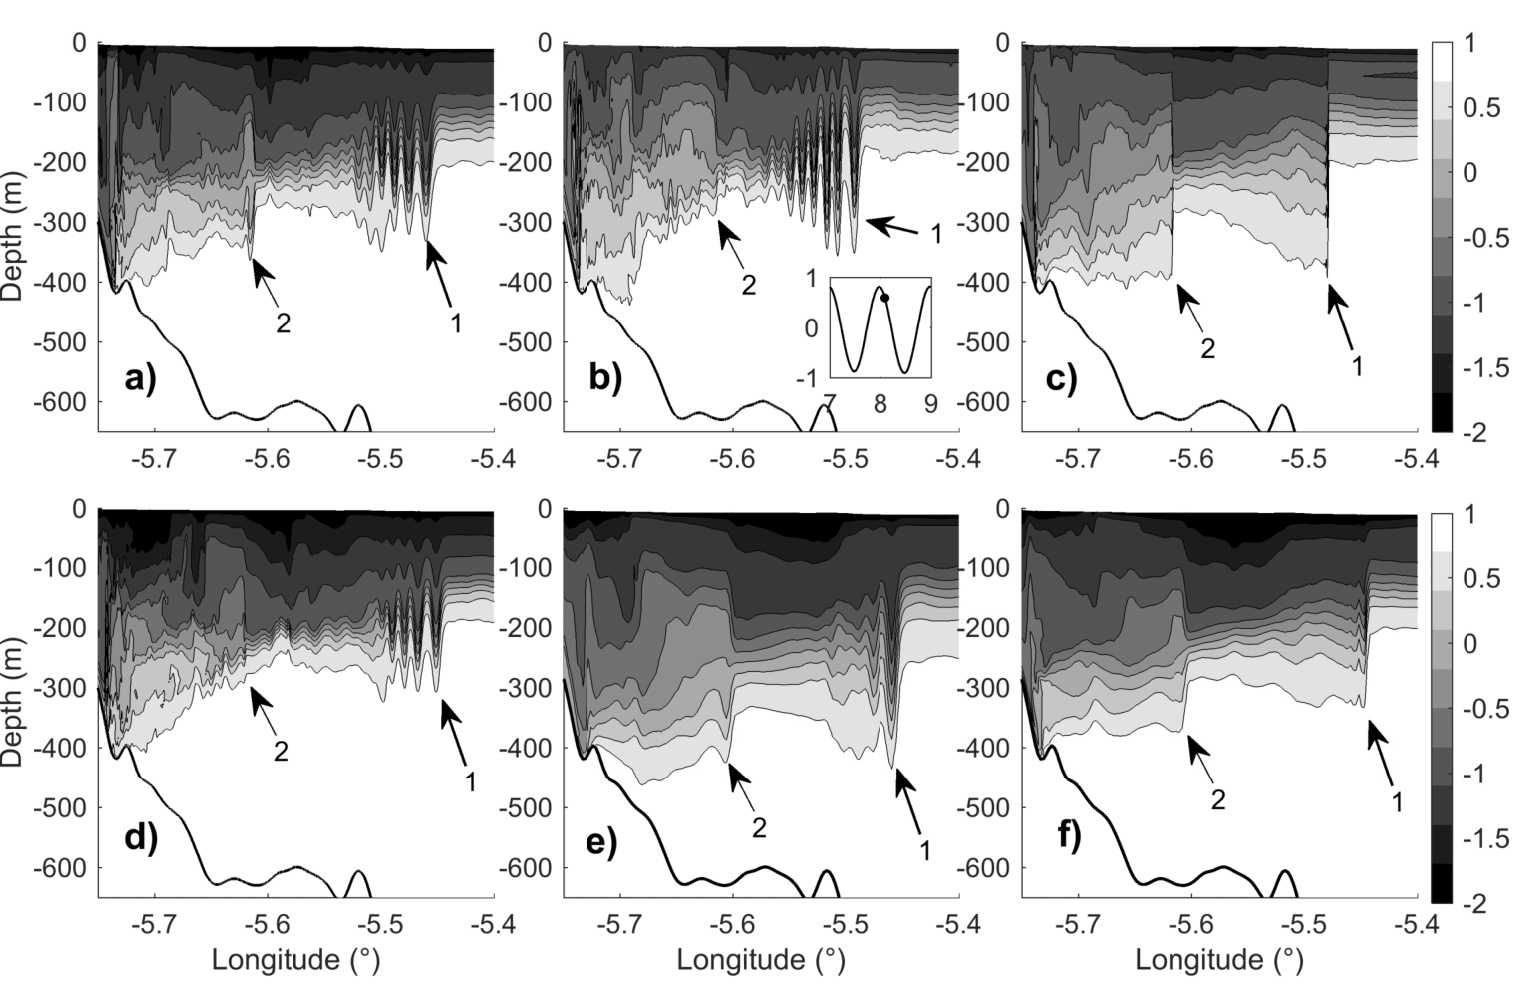
\includegraphics[width=\textwidth]{./GBR2D/figure12.png}
  \caption{Internal wave propagation from density field at $t = 8.1 T$ in (a) \textbf{SimRef}; (b) \textbf{SimW}; (c) \textbf{SimH}; (d) \textbf{SimV}; (e) \textbf{SimL}; and (f) \textbf{SimLH}. Large amplitude mode-1 waves (soliton or bore) are denoted as "1" and mode 2 as "2".}
  \label{fig_trains_num}
\end{figure}

As described in Section \ref{sisw}, mode-1 and mode-2 large amplitude internal waves are generated in the CS vicinity and propagate eastward during each ebb in all nonhydrostatic simulations. Figure \ref{fig_trains_num} presents the density fields in the region of the TN at $t\ =\ 8.1\ T$. A wave train with a minimum of two solitons can only be identified in the nonhydrostatic experiments. In the hydrostatic cases \textbf{SimH} and \textbf{SimLH}, the lack of nonhydrostatic dispersion produces internal waves propagating as internal bores. In the nonhydrostatic cases, these internal waves can propagate as trains of solitons with varying numbers of solitons (and celerity) : 6 in \textbf{SimRef}, 8 in \textbf{SimW}, 4 in \textbf{SimV}, and 2 in \textbf{SimL}. 

This illustrates a second aspect of the effect of hydrostatic assumptions, besides the inhibition of turbulent primary instabilities (KH instabilities in the region of the hydraulic jump). As already noted by previous authors \citep{Sannino2004}, the dispersion needed to balance nonlinear steepening in large-amplitude solitary waves is missing in hydrostatic simulations such as \textbf{SimH} and \textbf{SimLH} (Figure \ref{fig_trains_num}).

%---------------------------------------------------
\paragraph{Evolution of Stratification}
%---------------------------------------------------

\begin{figure}[!h]
\centering
  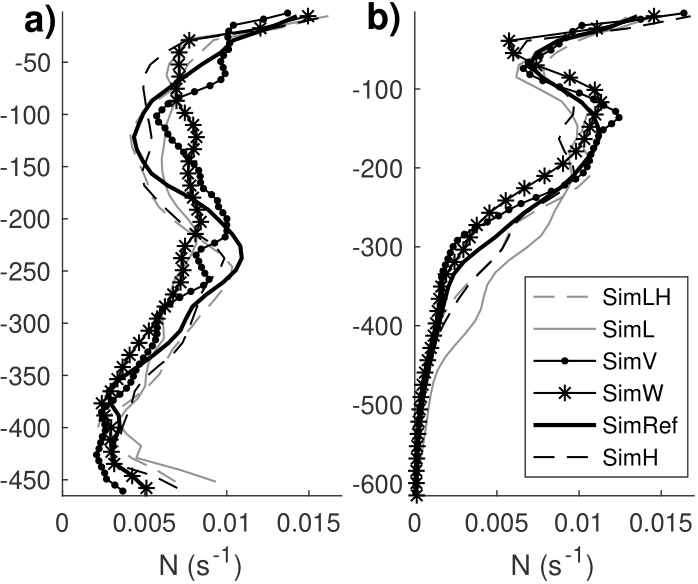
\includegraphics[width=0.7\textwidth]{./GBR2D/figure13.png}
  \caption {a) $N$ frequency computed at 5.8$^\circ$W longitude and time-averaged between 8.2 T and 8.7 T (during flood tide and presence of hydraulic jump). b) Same as (a) but at 5.55$^\circ$W longitude.}
	\label{fig_sensnum2}
\end{figure}

The previous results lead us to anticipate large differences in the way density stratification evolves in \textbf{SimRef}, \textbf{SimW}, \textbf{SimV}, \textbf{SimH}, \textbf{SimL}, or \textbf{SimLH}. To go further, Figure \ref{fig_sensnum2} shows for each configuration the profiles of Brunt-V\"ais\"al\"a frequency ($N$ defined in eq.\ref{eqN}) at 5.8$^\circ$W (a) and at 5.55$^\circ$W (b). Profiles are time-averaged over one flood. 

At 5.8$^\circ$W, stratification is similar in \textbf{SimH} and \textbf{SimLH} with an interface region (defined as the region where $N$ is maximal, here $N$ = 8.10$^{-3}$ s$^{-1}$) located at a depth of 250 m (Figure \ref{fig_sensnum2}.a). The nonhydrostatic simulations \textbf{SimRef} and \textbf{SimL} present an interface region at a similar depth but the vertical gradients are larger in \textbf{SimRef} and smaller in \textbf{SimL}.
\textbf{SimV} shows larger vertical gradients of density ($N$ = 1.1 10$^{-2}$ s$^{-1}$) and a shallower interface at a depth of 150 m. \textbf{SimW} is weakly stratified over most of the water column with no clear interface between the two water masses. This result may seem surprising because the WENO5 scheme is of fifth-order accuracy with more selective quasi-monotonic corrections near shocks than the TVD scheme, and is thus expected to produce less smoothing. This apparent contradiction can be explained by the generation of more intense primary shear instabilities (i.e. with higher values of associated vertical velocity and vertical velocity gradients), which has the effect of diffusing density gradients.

In Figure \ref{fig_sensnum2}.b, averaged $N$ profiles over one flood  are shown at 5.55$^\circ$W longitude in a region subjected to intense internal wave activity. \textbf{SimH}, \textbf{SimLH} and \textbf{SimL} exhibit similar profiles with $N$ slowly decreasing below the interface at 160 m. \textbf{SimRef} has a similar interface at 160 m but with higher $N$ value, although weaker stratification appear at the top of the lower layer. \textbf{SimV} and \textbf{SimW} both have shallower interfaces at 130 m, with $N$ reaching the highest values in \textbf{SimV} ($N$ = 1.25 10$^{-2}$ s$^{-1}$), as the enhanced vertical resolution allows the representation of stronger gradients.

Clear conclusions cannot yet be drawn concerning mixing. KH instabilities are expected in the region of the hydraulic jump and downstream. They lead to more stirring and consequently open up new opportunities to improve modelling of the route to mixing. Further investigation and diagnostics are now required to better understand the energy cascades. In particular, the present comparison between WENO5 and TVD advection schemes (and their implicit dissipation) indicates that numerical choices may unfortunately still have large consequences. Therefore, the role of physical and numerical closure must be considered comprehensively \citep{Marchesiello2011, Soufflet2016}.

%%%%%%%%%%%%%%%%%%%%%%%%%%%%%%%%%%%%%%%%%%%%%%%%%%%%%%%%%%%%%%%%%%%%%%%%%%%%%
\subsection{Discussion and Conclusion}
%%%%%%%%%%%%%%%%%%%%%%%%%%%%%%%%%%%%%%%%%%%%%%%%%%%%%%%%%%%%%%%%%%%%%%%%%%%%%

The present study focuses on small-scale dynamics in the Strait of Gibraltar and on the capacity of a new split-explicit, free-surface, nonhydrostatic regional oceanic model (CROCO) to represent such dynamics. Both objectives were pursued in parallel and several seminal results are obtained.

The study confirms that the generation of large-amplitude mode-1 and mode-2 internal waves in the Strait of Gibraltar as well as the onset of stratified turbulence and its energy cascade can be simulated with a computationally-efficient 2D vertical section. The characteristics of the simulated internal waves compare qualitatively well with published observations and previous numerical studies. Internal tides dynamics and shear instability in the hydraulic jump area are then analysed in more details, revealing characteristics and mechanisms.
 
The results of the study rely on a new type of nonhydrostatic, non-Boussinesq, free-surface kernel \citep{Auclair2018} implemented in the CROCO model. The resulting compressible oceanic model is presented in a realistic nonhydrostatic configuration for the first time. Sensitivity tests confirm that a nonhydrostatic (here non-Boussinesq) kernel is required (i) to simulate ISW trains and (ii) to explicitly simulate the onset of stratified turbulence energy cascade, provided that resolution is increased from about 200 m to 50 m. We conclude that resolutions finer than a few hundred meters are required in addition to a refinement of dynamical equations (relaxation of hydrostatic assumption) in order to solve the dominant dynamical processes in a key region of the Mediterranean.

Detailed characteristics of the vertical 2D configuration are also given with particular attention to the bathymetry and to the representation of the Coriolis force (implicit representation of funnelling effect in the strait). The proposed approach offers a computationally affordable way to make preliminary investigations of internal-wave dynamics in regions where these waves are important. However, the vertical 2D configuration is limited by the simplified representation of bathymetry and associated biases in the velocity shear between in-flowing Atlantic Waters and out-flowing Mediterranean waters. The inclusion of restratification processes (surface and boundary forcing) would allow the model to remain accurate for a greater number of tidal cycles --- the present configuration is considered accurate within three days after the spin-up period, before mixing starts to homogenise the water masses. Several remaining processes could not be considered: the transverse propagation of ISWs in the Strait of Gibraltar \citep{SG2011, vlasenko_2009} and in the Alboran Sea; the hydraulic control at the TN \citep{FA1988, Sannino2009b}; the boiling-water over the CS \citep{Bruno2002} or reflections on the strait's coasts. 

Only the ``onset'' of turbulence cascade could be simulated showing complex dynamics occurring in the area of the hydraulic jump at CS, with some small scale features identified as primary Kelvin-Helmholtz instabilities. Although this 2D study highlights how interesting this area can be, there is no doubt that simulation of secondary KH instabilities and subsequent energy cascade as well as the long term impact of these small scale processes on Mediterranean and North Atlantic circulation will require a fully 3D LES approach as well as dedicated field campaigns that explore these fine-scale processes.


%%%%%%%%%%%%%%%%%%%%%%%%%%%%%%%%%%%%%%%%%%%%%%%%%%%%%%%%%%%%%%%%%%%%%%%%%%%%%
%\appendix
%%%%%%%%%%%%%%%%%%%%%%%%%%%%%%%%%%%%%%%%%%%%%%%%%%%%%%%%%%%%%%%%%%%%%%%%%%%%%
\subsection{Appendix : evaluation of the first internal Rossby radius}
\label{app_Rossby}
%%%%%%%%%%%%%%%%%%%%%%%%%%%%%%%%%%%%%%%%%%%%%%%%%%%%%%%%%%%%%%%%%%%%%%%%%%%%%

The first internal Rossby radius is defined as :
\begin{equation}
\label{eqRosby}
R = \frac{\sqrt{g'h}}{f}
\end{equation} 
 At the Gibraltar Strait's latitude, the Coriolis parameter is $f=8.5 \times 10^{-5}\ s^{-1}$.
The numerator $c^{*}={\sqrt{g'h}}$ is the phase speed of the linear interfacial waves, into which the reduced gravity is:
\begin{equation}
g'= g \frac{\rho_M(S_M) - \rho_A(S_A)}{\rho_0}
\end{equation}
where $\rho_M(S_M) - \rho_A(S_A) \approx 2\ kg/m^{3}$. If the reference density is set to $\rho_0=1033.7\ kg/m^{3}$ and the gravity acceleration by $g=9.81\ m^2/s$, $g'=0.02\ m/s^{-2}$ which is in agreement with in situ data (cf \citet{Bryden94}). $h$ is a characteristic height given by:
\begin{equation}
h=\frac{h_1 h_2}{h_1+h_2}
\end{equation}
where $h_1$ and $h_2$ are respectively the upper and lower layer thicknesses. Picking up the data values from \citet{FA1988} (Table \ref{tabdepth}, first line), we obtain a range of $h = 50 - 100\ m$, which combined with the previous values for $g'$ and $f$ leads to $R$ ranging in 11.5 km (east of Camarinal Sill) to 16 km (west of Camarinal Sill). 

$\sqrt{g'h}$ can be replaced by the mode-1 internal waves speed($c_1$), which is estimated in the present study (\ref{app_Froude}) for the 3T-averaged stratification (\textbf{SimRef}) presented in Figure \ref{fig_fn_ref}. $c_1$ ranges between 0.8 m/s (at Camarinal Sill) and 1.8 m/s (in the eastern part of the strait), giving an estimated range of Rossby Radius ${c_1}/{f}$ between 9.5 and 21 km for the simulated section.


%%%%%%%%%%%%%%%%%%%%%%%%%%%%%%%%%%%%%%%%%%%%%%%%%%%%%%%%%%%%%%%%%%%%%%%%%%%%%
\subsection{Appendix : computation of a Froude number}
\label{app_Froude}
%%%%%%%%%%%%%%%%%%%%%%%%%%%%%%%%%%%%%%%%%%%%%%%%%%%%%%%%%%%%%%%%%%%%%%%%%%%%%
A single value of mode-n linear internal wave phase speed ($c_n$) can be computed for a flat-bottom and a linear stratification. This velocity can then be compared at each depth with the magnitude of local horizontal currents ($u$) to estimate when and where internal waves can propagate against currents. A diagnostic tool is the ratio of velocities, i.e. a Froude number $(F_n)$ defined as $F_n= u /c_n$. $c_n=\omega / k_n $ where $\omega$ is the wave frequency, here the M2-tidal frequency, and
%\begin{equation}
%\label{eqK}
%k_n=\pm \frac{n \pi}{H} \left( \frac{\omega^2 - f^2}{N^2 - \omega^2} \right) ^{1/2} 
%\end{equation}
$k_n$ are eigenvalues obtained by solving numerically the Sturm-Liouville problem associated with the linear propagation equation \citep{gill_atmosphere-ocean_1982}:
\begin{equation}
 W_n'' + k^2 \frac{N^2 - \omega^2}{\omega ^2 - f^2}W_n = 0
\end{equation}
with bottom and surface boundary conditions $W_n(0) = 0$ and $W_n(-H) = 0$. $W_n$ gives the structures of vertical modes. For each point on the x-axis, the profile N(z) is computed with Eq.\ref{eqN} from the 3T-averaged stratification in \textbf{SimRef} (shown in Figure \ref{fig_fn_ref}).

\begin{figure}[!h]
\centering
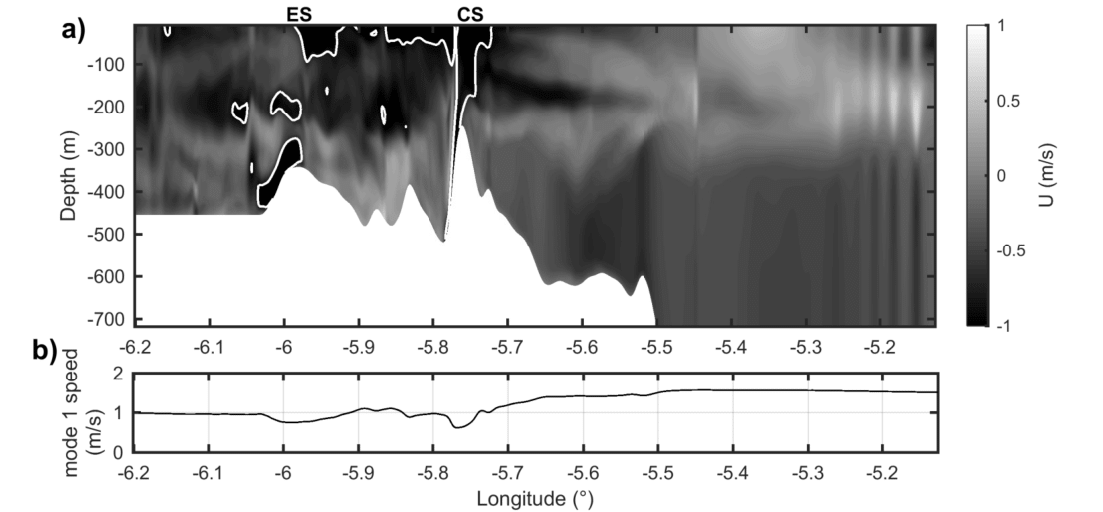
\includegraphics[width=1\linewidth]{./GBR2D/figure14.png}
\caption{a) Field of longitudinal velocity ($u (x,z)$) at $t = 8.5\ T$ with contours of mode-1 supercritical region (F$>$1) calculated from a 3T-averaged stratification. b) Computed speed of mode-1 linear internal waves ($c_1 (x)$) from a 3T-averaged stratification in configuration \textbf{SimRef}.}
\label{fig_annexeF}
\end{figure}

 The value of the first mode phase speed $c_1(x)$  is indicated in the lower panel of Figure \ref{fig_annexeF} and compared to the longitudinal velocity $u(x,z)$ at $t = 8.5\ T$ plotted in the upper panel. The areas where $u(x,z) > c_1 (x)$ (equivalent to Froude number $F_1$ larger than 1) are presented in the upper panel as well. The flow inside those contours is called supercritical.
 
 %%%%%%%%%%%%%%%%%%%%%%%%%%%%%%%%%%%%%%%%%%%%%%%%%%%%%%%%%%%%%%%%%
 \subsection{Appendix : computation of Okubo-Weiss parameter}
 \label{annexeOW}
 %%%%%%%%%%%%%%%%%%%%%%%%%%%%%%%%%%%%%%%%%%%%%%%%%%%%%%%%%%%%%%%%%
The Okubo-Weiss parameter (OW) is defined as
\begin{equation}
OW=s_n^2+s_s^2-\Omega^2
\label{eqOW}
\end{equation}
With $s_n$ the normal strain component, $s_s$ the shear strain component and $\Omega$ the vorticity. Usually, it is used in a xy-plane (e.g., for tracking eddies in \citet{Chelton2007}), but it is computed here in the zx-plane with the strains and vorticity expressed as :
\begin{equation}
s_n = \frac{\partial w}{\partial z} - \frac{\partial u}{\partial x} \quad , \quad
s_s = \frac{\partial u}{\partial z} + \frac{\partial w}{\partial x} \quad , \quad
\omega = \frac{\partial u}{\partial z} - \frac{\partial w}{\partial x}
\end{equation}
Negative values of OW indicate a greater role of rotation over deformation, and thus the presence of coherent vortices.

 %%%%%%%%%%%%%%%%%%%%%%%%%%%%%%%%%%%%%%%%%%%%%%%%%%%%%%%%%%%%%%%%%
\subsection{Appendix : a Korteweg-de Vries (KdV) model}
\label{KdVpart}
%%%%%%%%%%%%%%%%%%%%%%%%%%%%%%%%%%%%%%%%%%%%%%%%%%%%%%%%%%%%%%%%%%%%%%
\begin{figure}[!h]
\centering
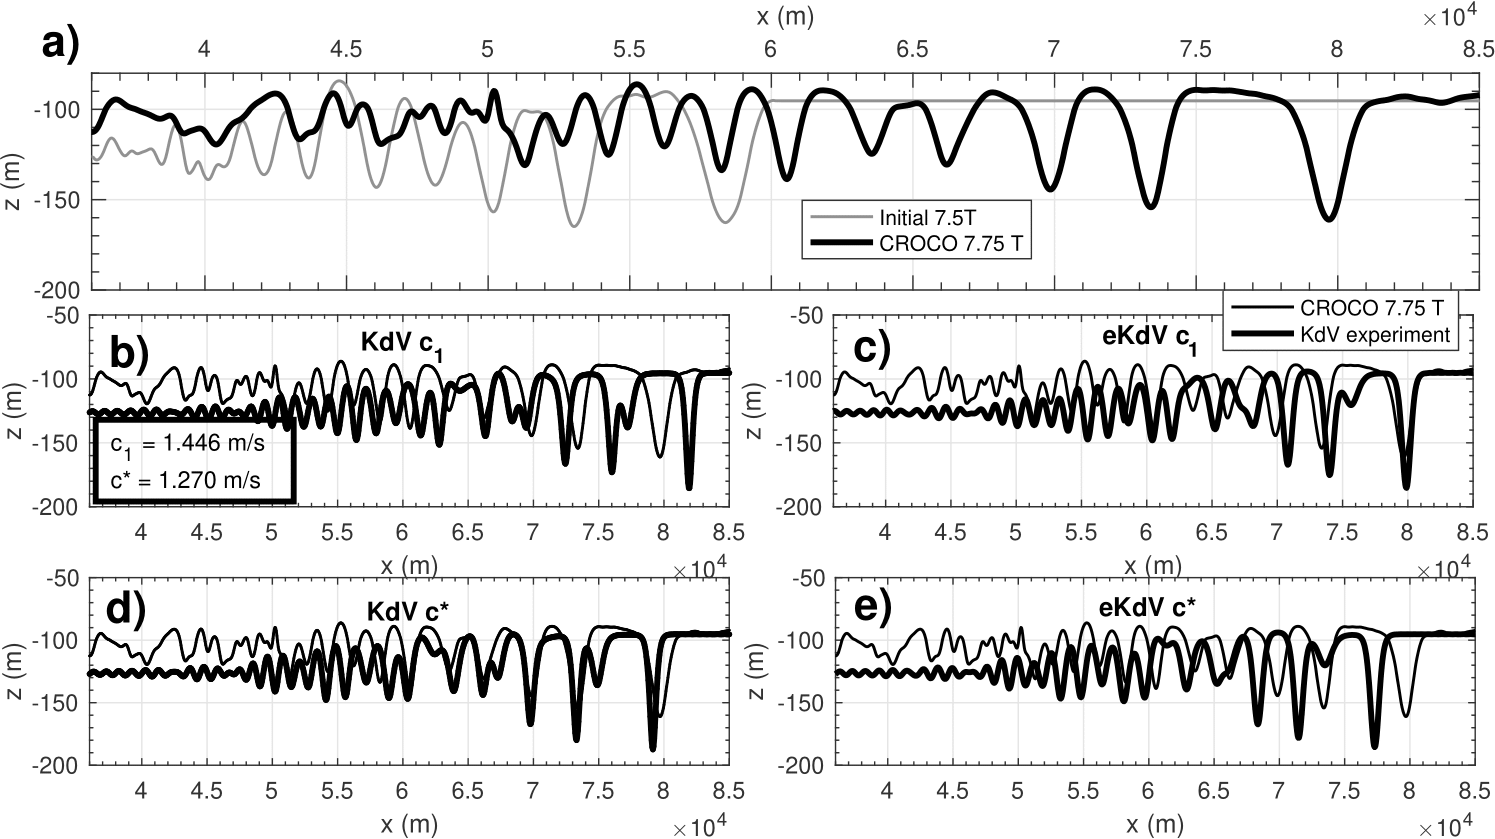
\includegraphics[width=1\linewidth]{./GBR2D/figure15.png}
\caption{ a) Isopycnal $\rho$'\ =\ -0.2\ kg/m$^3$ simulated by CROCO in \textbf{SimRef+} at $t\ =\ 7.5\ T$ (grey line; the interface depth is left constant downstream of the wave) and at $t\ =\ 7.75\ T$ (black line). b-e) Evolution of the interface simulated by KdV or eKdV (bold) and \textbf{SimRef+} (solid line) at $t\ =\ 7.75\ T$. Two propagation speeds are used: c$^*$ (d,e) and c$_1$ (b,c) (see text for details).}
\label{fig_kdv}
\end{figure}

Following many studies \citep{SG2008, Sannino2009b, vlasenko_2009}, the large amplitude internal waves of Section \ref{sisw} are termed ''ISWs'' for Internal Solitary Waves. To confirm that the internal waves observed in this section are ISWs, they are now compared with solutions of the Korteweg-de Vries equation which is recalled below. The solutions of this equation satisfy a balance between nonhydrostatic dispersion and nonlinear advection. Nonlinear advection steepens the wave front, whereas nonhydrostatic dispersion reduces steepening by transferring energy from large to small scales, resulting in a relatively stable entity called a ''solitary'' wave, or soliton.

The Korteweg-de Vries (KdV) equation describes the evolution of an infinitely thin interface in a two-layer system with constant bottom topography:
\begin{equation}
\frac{\partial \zeta}{\partial t} 
+c^* \frac{\partial \zeta}{\partial x}
\underbrace{+ \frac{3}{2} \frac{h_1-h_2}{h_1h_2} c^* \zeta \frac{\partial \zeta}{\partial x} }_{A}
\underbrace{+ \frac{1}{6} h_1h_2c^* \frac{\partial ^3 \zeta}{\partial x^3} }_{B}
\underbrace{ - \frac{3}{8}\zeta^2c^*\frac{h_1^2+6h_1h_2+h_2^2}{8(h_1h_2)^2} }_{C}
=0
\label{eq_kdv}
\end{equation}
where $c^*$ is the interfacial speed of small-amplitude internal waves: $c^*=\sqrt{g' h}\ = \ R.f$ and $\zeta$ is the vertical displacement of the interface. $g'$ and $h$ have already been defined in \ref{app_Rossby}.
%
The first two terms on the left-hand-side of (\ref{eq_kdv}) are those involved in the classical propagation equation for a small-amplitude, linear, interfacial wave travelling in the x-direction at speed $c^*$. The third term (bracket A) is a first-order approximation (with respect to amplitude) of nonlinear advection. Term (B) is a dispersive term.
%
The fifth term (C) is a higher-order non-linear term associated with a second order development for advection. The complete equation (\ref{eq_kdv}) will be referred to as "extended KdV" (or "eKdV"), whereas the same equation without term (C) will simply be referred to as "KdV" \citep{Dossmann2012}.

The simulated large amplitude waves presented in this study are compared with the solutions of the KdV or eKdV equation to gain insight into their dynamics. For optimal comparison, a new simulation, called \textbf{SimRef+} was carried out. Its characteristics are similar to \textbf{SimRef} (Table \ref{tabsimref}), except that (i) the eastern boundary is shifted 42-km to the east into the Mediterranean sea and (ii) the tidal forcing is stopped after only 7.25 periods. The first eastward-propagating train of mode-1 waves generated by the tide at the CS is compared with the propagation given by numerical integration of the KdV and eKdV equations (eq. \ref{eq_kdv}).

The vertical displacement of isopycnal $\rho'\ =\ -0.5\ kg/m^3$ is extracted\footnote{Due to the extension of the domain to the east, a new value of $\rho_0$ is computed : $\rho_0\ =\ 1033.9 \ kg/m^3$ to optimize computations.} at $t_0\ =\ 7.5\ T$ when the mode-1 ISW train propagates over a region of constant depth ($H\ =\ 890\ m$) east of TN (Figure \ref{fig_kdv}), so as to get closer to the KdV framework. The position of the chosen isopycnal surface at this time is shown in Figure \ref{fig_kdv}.a. At that time, the distance between the first and second solitons of the train is 5 km; the first soliton has an amplitude of 75 m and the train includes 7 solitons. This isopycnal is chosen as initial state for the KdV or eKdV model. 
%
The KdV and eKdV equations are integrated either with the interfacial wave speed ($c^* \approx 1.27\ m/s$) or with mode-1 velocity ($c_1 = 1.45\ m/s$; see \ref{app_Froude} for details on $c_1$ evaluation).

Figures \ref{fig_kdv}.b-e compare the interface depth obtained at $t\ =\ t_0\ +\ 0.25\ T$ in the KdV and eKdV models with the position of the $-0.5\ kg/m^3$ isopycnal in \textbf{SimRef+}. In the latter, the distance between the first two solitons has grown since $t =\ t_0$ and reaches 7 km with an amplitude of 70 m for the first trough. The train is now made of 11 solitons: the first three have decreasing amplitudes, then two smaller solitons of comparable amplitude (40 m) and one soliton of greater amplitude, followed by solitons with decreasing amplitude again. 

In the KdV solution obtained with propagation speed c$^*$ the first solitary wave is slightly slower but its amplitude is markedly larger (Figure \ref{fig_kdv}.d). The remaining solitons of the train are well located, but a secondary trough is generated between the first two solitons whereas it is absent in \textbf{SimRef+}.

Using the larger mode-1 speed $c_1$ instead of $c^*$ (Figure \ref{fig_kdv}.b), the train of solitons in KdV is too fast. When the eKdV equation is used with speed $c^*$ (e), the solitons are too slow, whereas this same extended equation with $c_1$ (c) leads to a correct displacement of the solitons. 
Overall, the temporal evolution of solitary waves in \textbf{SimRef+} is consistent with the solutions of the KdV or eKdV equation (\ref{eq_kdv}). However, the KdV or eKdV framework remains an inviscid simplification. Note that closer evolution of soliton amplitudes between KdV or eKdV and \textbf{SimRef+} solutions can be obtained by simply adding a diffusive term in KdV or eKdV equation. This also slows down propagation in KdV, and to a lesser extent in eKdV (not shown).

The KdV or eKdV model also involves adjustable parameters, such as the linear wave speed, which ranges between the interfacial speed $c^*$ and the mode-1 speed $c_1$, each being one particular approximation of the wave's behaviour. 

That being said, the wave trains in \textbf{SimRef+} are appropriately modeled as KdV or eKdV ISWs, which confirms (i) the propagation of interfacial troughs as trains of solitons and (ii) CROCO's ability to simulate the subtle balance between nonhydrostatic effects (responsible for dispersion) and nonlinear advection. 
 
%%%%%%%%%%%%%%%%%%%%%%%%%%%%%%%%%%%%%%%%%%%%%%%%%%%%

\paragraph{Acknowledgments} This work was partly funded by the DGA "Etude Amont" Protevs driven by the Shom. It was granted access to the HPC ressources of CALMIP supercomputing center under the allocation P18017. We also gratefully thank the computer team of the \textit{Laboratoire d'Aérologie} for its support. Margaux Hilt's PhD thesis was funded by a MESRI scholarship. 


%\bibliography{biblio_gib_doi}

%\end{document}
